\documentclass[a4paper]{article}

%% Language and font encodings
\usepackage[english]{babel}
\usepackage[utf8x]{inputenc}
\usepackage[T1]{fontenc}

%% Sets page size and margins
\usepackage[a4paper,top=2cm,bottom=4cm,left=1cm,right=7cm,marginparwidth=6cm]{geometry}

%% Useful packages
\usepackage{amsmath}
\usepackage{amssymb}
\usepackage{bm}
\usepackage{wrapfig}
\usepackage{float}
\usepackage{graphicx}
\usepackage[colorinlistoftodos]{todonotes}
\usepackage[colorlinks=true, allcolors=blue]{hyperref}
\renewcommand{\familydefault}{\sfdefault}
\usepackage{hyperref}
\usepackage{algorithm}
\usepackage[noend]{algpseudocode}

\newcommand{\introduce}[1]{%
  \leavevmode % if at the start of a paragraph
  \marginpar{\small\emph{#1}}% the note
}

\newcommand{\ix}[1]{%
  \leavevmode % if at the start of a paragraph
  \marginpar{\small\emph{#1}}% the note
}

\newcommand{\iix}[1]{%
  \text{#1}
  \leavevmode % if at the start of a paragraph
  \marginpar{\small\emph{#1}}% the note
}

\newcommand{\marfig}[2]{
  \marginpar{ \includegraphics[width=\marginparwidth]{#1} \centering \text{#2} }
}

\newcommand{\vect}[1]{\boldsymbol{\mathbf{#1}}}

\newcommand{\myfig}[4]{
  \begin{figure}[H]
  \centering
  \includegraphics[width=#4\textwidth]{#1}
  \label{#2}
  \caption{#3}
  \end{figure}
}

\renewcommand\labelitemi{$\bullet$}

\title{\textbf{3G4 Medical Imaging \& 3D Computer Graphics}\\
\textit{Course Notes}
}
\author{Mrinank Sharma}

\begin{document}
\maketitle
% \tableofcontents
Please note that the margins of these notes can be used to check factual recall simply by covering up the right hand text.

\section{Medical Image Acquistion}
\subsection{Ultrasound}
\ix{Principles of Ultrasound}Ultrasound imaging works by firing high frequency sound waves into the body. Ultrasound imaging is used for imaging tissue alone; often layers of air may prevent wave transmission and a gel can be applied to the skin. The ultrasound waves interact in complex ways: \ix{Wave Interaction}
\begin{enumerate}
  \item Attenuation occurs due to viscosity which converts acoustic energy to heat. 
  \begin{align*}
    A_z = H(f, z)A_0 \text{ where } H(f, z) = e^{-\alpha_0 f^n z}
  \end{align*}
  \(\alpha = \alpha_0 f^n\) has units of $\text{Np cm}^{-1}$ where a Np is a dimensionless unit. In general, the lower the frequency, the better the penetration. 

  \item Reflection and refraction occur. Define $k=\omega / c$ and $Z=\rho c$ as the acoustic impedence. Then
  
  \marfig{waveRefraction}{}

  \begin{align*}
    R = \frac{I_r}{I_i} = \Big(\frac{Z_2 - Z_1}{Z_2 + Z_1}\Big)^2 \hspace{1cm} T = \frac{I_t}{I_i} = \frac{4Z_1Z_2}{(Z_2 + Z_1)^2}
  \end{align*}
  \textbf{N.B.} Intensity is analogous to power. Thus use $10 \log \alpha$ for dB.
\end{enumerate}

\ix{Signal Processing - What \& Why?}A 1D image, known as a \emph{A-line} can be obtained by sending a pulse using the piezoelectric crystal array which acts as both the transmitter and receiver. The resulting signal is processed as follows:
\begin{enumerate}
  \item Low-pass filtering and envelope detection to clean the signal. This removes high frequency noise and uninteresting RF oscillations.
  \item Time gain compensation: the ultrasound wave is attenuated by tissue. If the material was homogenous, an exponential correction would be applied but since there are normally different tissues in the image, most scanners allow the user to special the TGC curve.
  \item Log-compression: this compensates for the amplitude difference between specular and scatter reflections without which speckle would not be visible. This \emph{stretches the range of small reflections and compresses the range of larger reflections}.
\end{enumerate} 

\ix{A-lines and B-scans}By electronically scanning multiple 1D images (A-lines, for which the signal \emph{envelope} is used) a full 2D B-scan can be constructed. The temporal resolution is excellent with $\approx 75$ B-scans per second. 

\ix{Doppler Imaging}Motion \textbf{parallel} to the wave can be measured using \emph{Doppler Imaging}. This tends to have inferior spatial and temporal resolution than normal ultrasound. There are two forms of Doppler imaging:
\begin{enumerate}
  \item Continuous Wave doppler imaging measures the frequency shift of a continuous wave transmitted into the body and it unable to detect velocity locations.
  \item Pulsed Wave doppler imaging fires a short sequence of pulses on the same line and looks at the phase differences between the received signals. This can be used to construct colour flow images.
\end{enumerate}

\ix{M-Mode Imaging}Motion mode imaging repeatedly scans a single A-line and displays the 1D image against time. This is used for structures moving at speeds higher than the B scan rate. 

\ix{Waves}The piezoelectric crystal which deform when placed in an electric field have a high frequency AC voltage applied which when placed to the patients skin cause the vibration to spread. Eventually, an equilibrium is reached with all particles vibrating but this can be viewed as a \emph{propagating longnitudinal pressure wave} with rarefactions and compressions. 
\begin{align*}
  \frac{\partial^2p}{\partial x^2} =& \frac{1}{c_0^2} \frac{\partial^2p}{\partial t^2} \\ 
  p(x,t) =& A_1 f_1(x-c_0 t) + A_2 f_2(x+c_0 t)
\end{align*}
The solution is two arbitrary waves propagating left and right. Note that
\begin{align*}
  c_0 =\frac{1}{\sqrt{\rho_0 \beta_0}} \text{ where the adiabatic compressibility is given by } \beta=\frac{1}{\rho} \frac{\partial \rho}{\partial p}
\end{align*}
Whilst different tissues thus have different speeds, the scanner assumes an average speed of \(1540\ ms^{-1}\).

\ix{Image Features}Due to the properties of ultrasound, their images often have common features:
\begin{enumerate}
  \item Dark regions at the `bottom' of images are caused by attenuated. 
  \item Clear boundaries between different tissue types are caused by specular reflection and refraction. 
  \item Speckle patterns are due to scattering. 
  \item Enhancement artifacts may also occur where the wave has passed through a low attenuation material resulting in following features producing stronger echos. 
\end{enumerate}

\ix{Axial Resolution}The axial resolution is \(w/2\) where \(w\) is the pulse width (in space) (e.g.\ try to find an object of length \(w/2\)). Since at least time period must be transmitted, the width is larger for lower frequencies and this the resolution is better with higher frequencies.

\ix{Lateral Resolution}Multiple transducer elements fire at once, appropriated delayed, to achieve a good lateral resolution. The image on the left fixed the depth but \textbf{dynamic receive focusing} allows appropriate focusing at different depths by constantly adjusting the focus delays.

\begin{figure}[H]
  \centering
  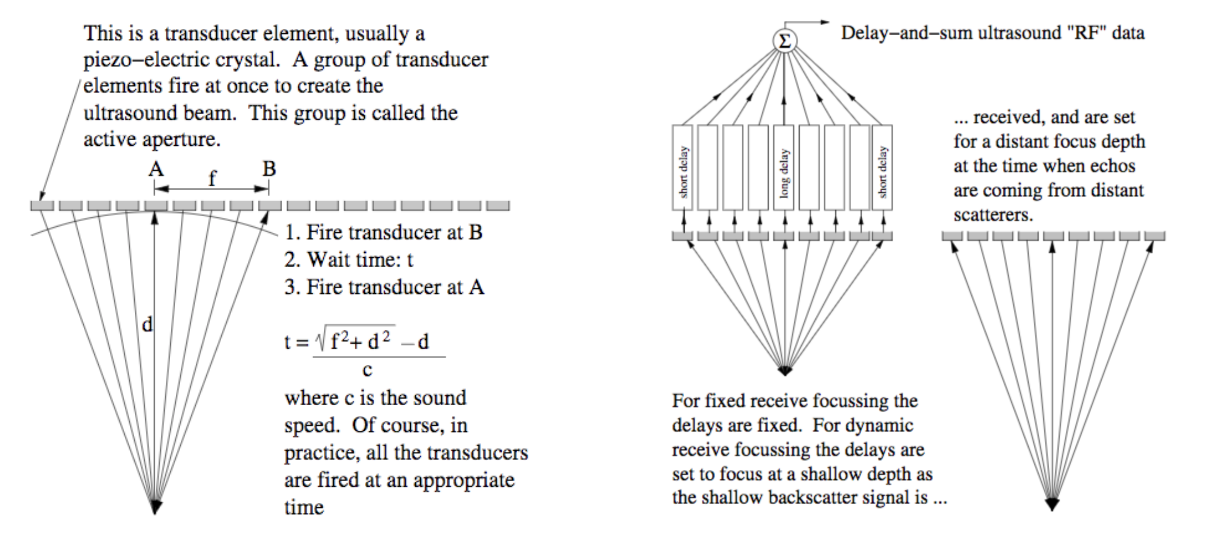
\includegraphics[width=\textwidth]{latRes}
\end{figure}

\ix{Elevational Resolution}An acoustic lens is often used to focus in the elevational direction (for both transmit and receive). Some modern machines have rows of transducer elements in the elevational direction and thus achieve this focus using delays (2.5D imaging).

\ix{Scatter reflections}Small local variations of density and compressibility give rise to scatter reflections. Point scatters retransmit incident waves in all directions. The waves which head back to the probe and known as backscatter. Within each resolution cell, there are many scatters and the scanner sums the individual backscatter wavelets and thus we have the characteristic noise. 

\ix{3D Ultrasound - the options}There are many ways to obtain 3D ultrasound data.
\begin{enumerate}
  \item Oscillating head probes (a normal probe mounted on a motor) acquire rotational or fan shapes volumes. These are easy to use since they produce evenly sampled data (which can be resliced), positionally accurate and available commercially but they only acquire a fixed, small volume. 
  \item 2D phased array transducers acquire pyramid shapes volumes as the crystal matrix steer the beam. Conversion is difficult with many crystals and cabling. 
  \item Freehand scanning allows the area of interest to be scanned with the position tracked using an additional device. Whilst there is no limit to the volume size acquired or it's shape, the position sensor requires careful calibration and unevenly sampled data can be produced which is challenging to work with. 
\end{enumerate}

\subsection{X-Rays}
X-Rays normally produce projection images but through rotation, a full 2D slice can be produced (CT). X-rays are a form of EM radiation and this with a wavelength of the order \(10^{-10}\), the photon energies tend to be around \(100 keV\). \ix{Generation} X-Rays are generated by bombarding a \emph{tungsten} anode with electrons which are produced using a heated filament. 

\marfig{xraygen}{}

Above, the anode rotates to help to dissipate heat\ix{Rotation: why?} since only $1\%$ of the electron energy goes into X-rays. A spectrum of X-rays is generated.

\ix{Why peaks in the spectrum?}
\begin{figure}[H]
  \centering
  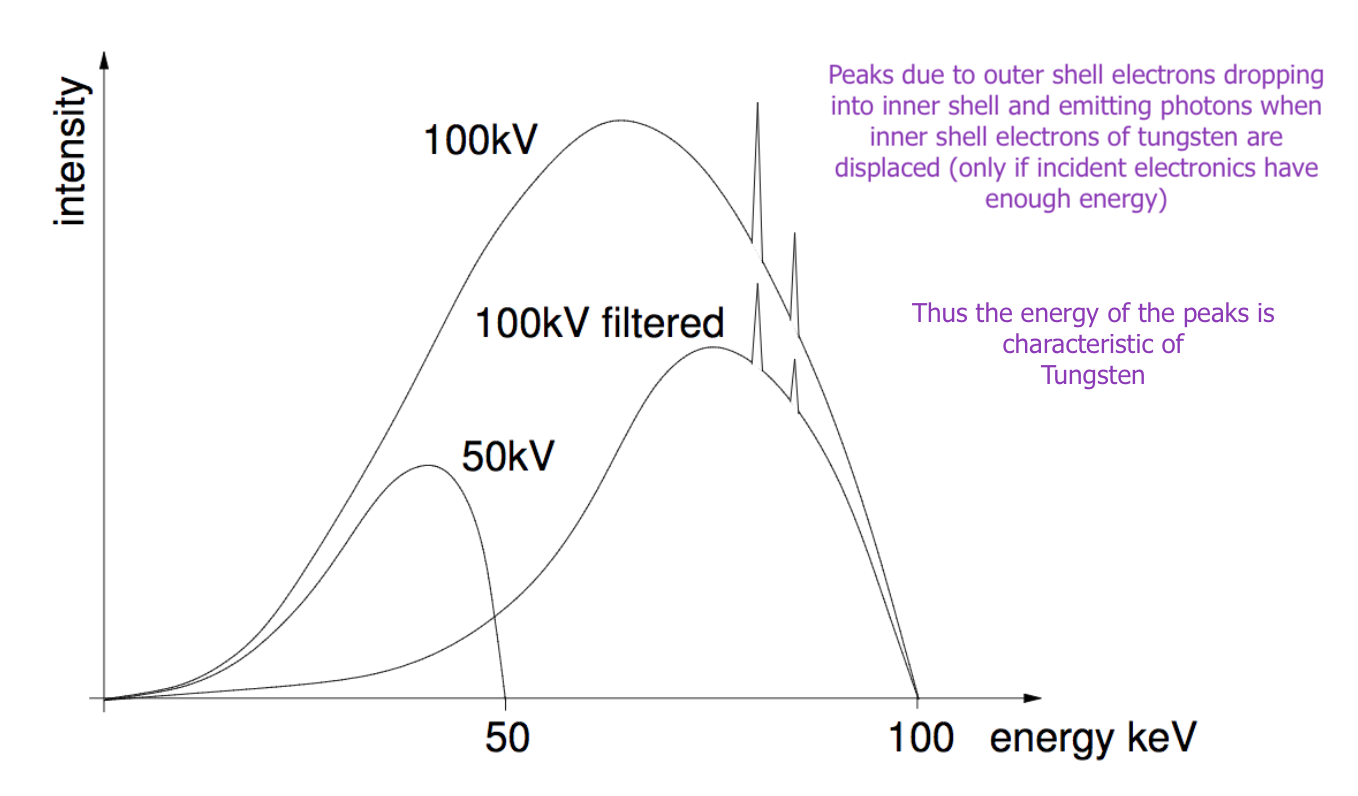
\includegraphics[width=0.8\textwidth]{xraygenspc}
\end{figure}

X-rays\ix{Attenuation. What controls \(\mu\)} are attenuated when they pass through media 
\begin{align*}
  I = I_0 e^{-\mu x} \text{ or } I = I_0 e^{-\int\mu (x) dx} \text{ for continuous media}
\end{align*}
Where \(\mu\) depends on the photon energy, material atomic number and density. There are two main types of attenuation.

\ix{Attenuation types?}
\begin{figure}[H]
  \centering
  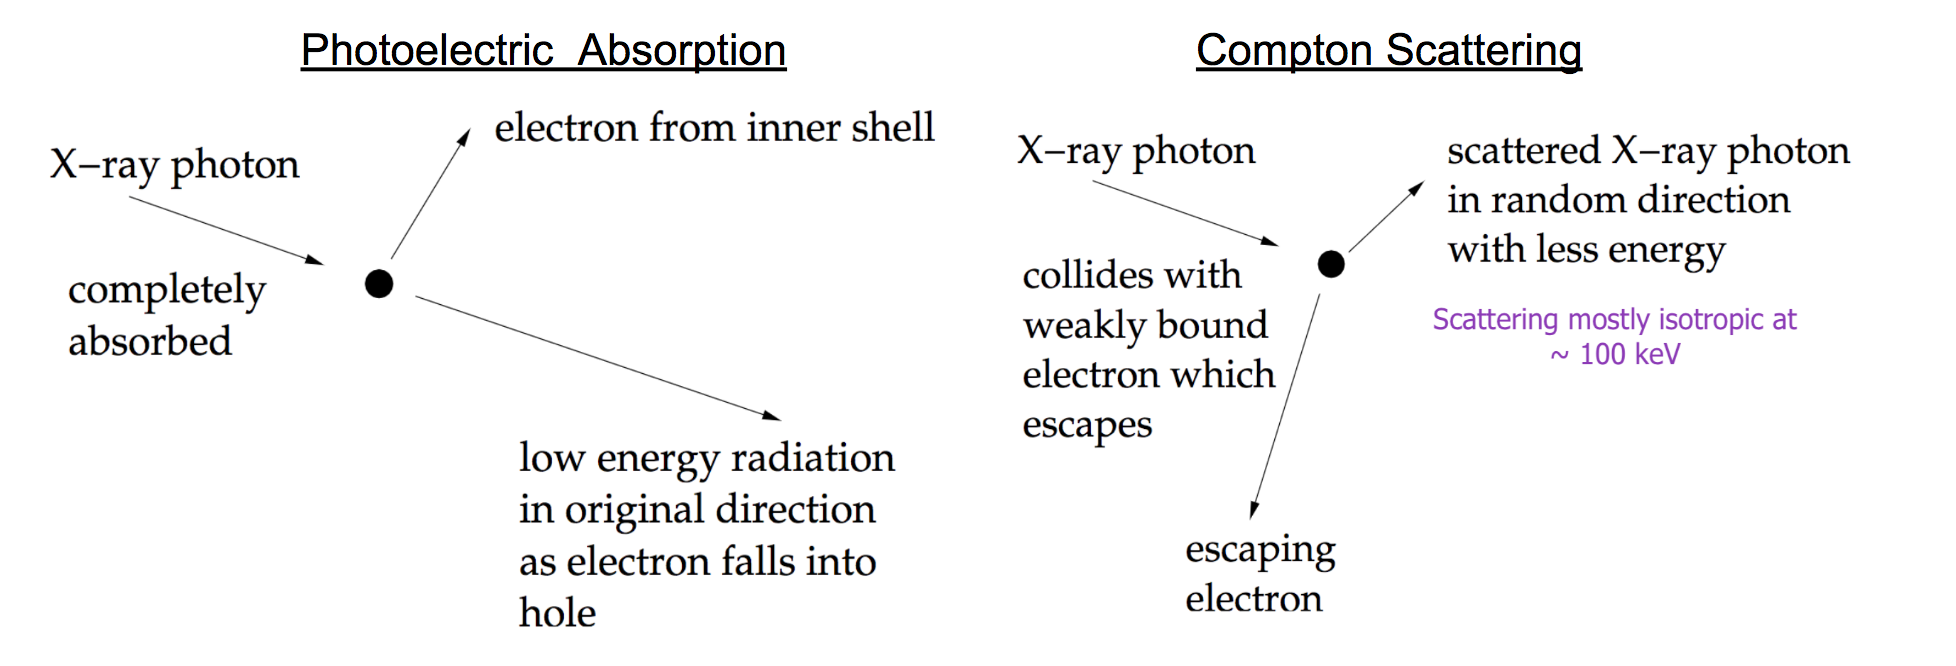
\includegraphics[width=\textwidth]{xrayatt}
\end{figure}

\ix{Beam Hardening}X-rays of higher energy are more penetrating. Thus the deeper an X-ray penetrates, the more the spectrum bunches to the higher energy end of the scale. This is known as \textbf{beam hardening}. \ix{Pre-hardening: why?}The superficial absorption of lower energy photons increases the radiation dosage and only distorts the output; thus a filer of \texttt{Al} or \texttt{Cu} (a beam-hardening filter) is used to pre-harden the beam.

When a screen-film detector is used, an emulsion of gelatine with suspended silver bromide is used. \(3-10\%\) of the X-ray energy is absorbed by the emulsion. Intensifying screens are used to increase the sensitivity (these screens fluoresce when stimulated by X-rays, produced visible and UV light) as is a reflective layer of \texttt{TiO\textsc{2}}. 

\ix{Scintillation Crystal Photomultiplier Coupled Detector}
A Scintillation Crystal Photomultiplier Coupled Detector has an output voltage proportional to the energy of the incoming X-ray photon. The initial light is produced as X-rays are attenuated and the flashes are then amplified millions of times. This detector is fast and efficient but has a low packing density. 

\begin{figure}[H]
  \centering
  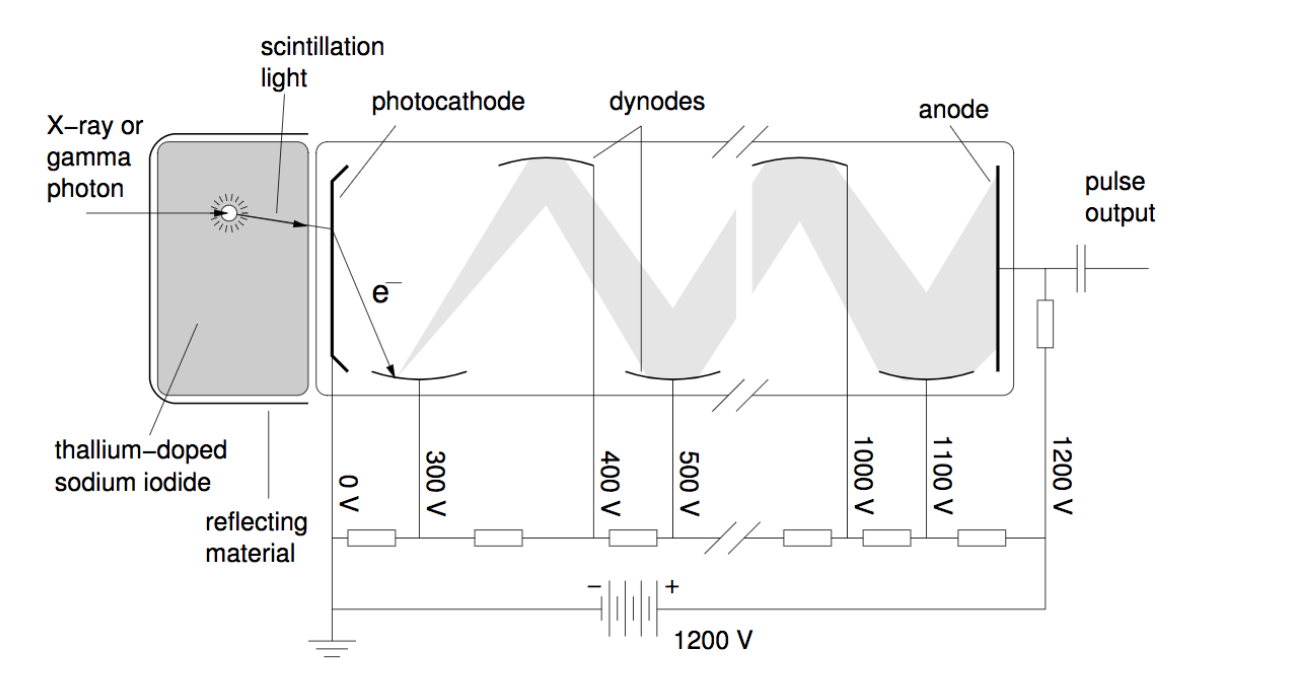
\includegraphics[width=0.8\textwidth]{xraydet}
\end{figure}

There also exist other detectors such as scintillation crystal-photodiode coupled (scintillaton light detected by a photodiode, fed to a amplifier) which is fast, high efficiency and densely packed. Can also use gas ionisation detectors where Xenon gas is ionised by x-rays, causing ions to be drawn to the electrodes which produce a current. Simple but slow and low efficiency.

CT scanners are able to produce a full 2D image where each pixel represents the CT number of the body at that point. A 2D image is produced using multiple coplanar scans at different angles. 
\begin{align*}
  \text{CT Number (Hu)} = \frac{\mu - \mu_{\text{H}_2\text{O}}}{\mu_{\text{H}_2\text{O}}}\times 1000  
\end{align*}
\ix{Grey-Level Transformation} There is a high dynamic range in the CT number and hence a suitable transform must be applied. CT scans are HD, cheap and fast but involve large doses of X-rays. 

We seek to find the attenuation field, \(\mu(x,y)\) but the scanning method produces a rotated coordinate system \((s, l)\) which can be seen by considering the diagram found on the right. \marfig{rotCords}{Rotated Coordinates} For a fixed angle, the measured profile is given by
\begin{align*}
  I_{\phi}(s)=I_0 \exp [-\int\mu(x, y)\ dl]
\end{align*}
This may be transformed into an attenuation profile which is the \emph{projection} of \(\mu\).
\begin{align*}
  p_\phi (s) &= - \log \frac{I_{\phi}(s)}{I_0} \\
  p(s, \phi) &= p(-s, \phi \pm \pi) \text{ (symmetry)}
\end{align*}

By taking the\ix{Forming the Sinogram \& The Radon Transform} full set of projections at different \(\phi\) a 2D \emph{sinogram} can be formed. \marfig{sinugram}{A Typical Sinogram}The name can be understood by considering the sinogram of a single point. The \emph{Radon Transform} maps a function into its sinogram (i.e. to sets of integrals over lines perpendicular to an angle of \(\phi\) at distance \(s\) from the origin.)
\begin{align*}
  \mathcal{R}[f(\vect{r})] = \int_{\vect{r.u}=s} f(\vect{r})\ |d\vect{r}|
\end{align*}
Thus we seek to find a way of inverting the Radon transform. By considering the one-dimensional Fourier transform of the projection data and applying a coordinate transform and then noting the form of the 2D fourier transform, we form the \emph{projection theorem}. \ix{(Proving) The Projection Theorem}
\begin{align*}
  \mathcal{F}_1[p_{\phi}(s)](\omega) = \mathcal{F}_2[\mu(x, y)](\omega \cos (\phi), \omega \sin (\phi) )
\end{align*}
Thus the \emph{1D Fourier Transform of the projection data is the same as the radial data of the 2D Fourier Transform of \(\mu(x, y)\)}. This forms the basis of the direct fourier reconstruction algorithm. 

\myfig{directFourier}{}{Direct Fourier Reconstruction}{0.6}

\ix{Issues}This relies on an accurate 2D algorithm for interpolation. An alternative is \emph{filtered backprojection}. This may be derived by using the projection theorem, inverting \ix{(Proving) Filtered Backprojection} the 2D Fourier transform then applying a change of coordinate system. Noting that the inner integral is a one-dimensional inverse fourier transform in the s direction and that multiplication in frequency is convolution in space, we find that \marfig{backProj}{Filtered Backprojection}
\begin{align*}
  \mu(x, y) &= \int_{0}^{\pi} p_\phi(s) * q(s)\  d\phi \text{ where } q(s) = \mathcal{F}_{1}^{-1}[|\omega|](s) \\
  \mu(x, y) &= \sum \mu_i(x, y) \text{ where } \mu_i(x, y) = p_{i\Delta\phi}(s) * q(s)
\end{align*}
Note that \emph{the form of} \(\mu_i\) \emph{implies that each projection is `smeared' backwards then summed} since each \(\mu_i = \mu_i(s)\). In reality, the filter kernel is divergent in frequency but since each X-ray has finite width, the maximum \textbf{spatial} frequency is \(2\pi / t\) meaning that the filter can be cut off. \marfig{ramLak}{Ram-Lak Filter}Often a smoothing window (e.g. Hamming) is applied to the filter. Note that the beam width also determines the minimum detector spacing to limit aliasing. 

\ix{CT Artifacts} CT Artifacts are caused by under-sampling, beam hardening and scatter. Beam hardening often exhibit streak artefacts e.g. when scanning the brain, only higher energy photons pass through which are then attenuated less, giving a low value of \(\mu\) and thus streaks. Cupping also occurs - reduced attenuation in the centre of objects. Furthermore, the X-ray source is likely poly-chromatic. 

\ix{Scanning Strategies}There are several strategies for CT scans.
\begin{enumerate}
  \item First Generation: a single detector is translated across a subject. The detector unit then rotates and the scan is repeated. (5 min per slice)
  \item Second Generation: A fan beam is used with multiple detectors, decreasing scan time (\(20s\) per slice).
  \item Third Generation: A wider beam and a detector array is used which covers the entire FoV. Only rotation required (\(0.5s\) per slice). This is the most successful generation.
  \item Fourth Generation: the X-ray tube rotates with a fixed array of detectors. 
\end{enumerate}

Similarly,\ix{3D CT Scanning Strategies} there are several strategies to produce 3D data:
\begin{enumerate}
  \item Sequential CT:\ scan planes sequentially using a motorised table. The step size is determined by the Nyquist criterion and the slice thickness.
  \item Spiral CT:\ the table is moved continuously as the detector rotates. Interpolation required.
  \item Multislice CT:\ Several planes are scanned at once by using a fat beam with multiple detector arrays.
  \item Cone-beam CT:\ A very wide beam and a full 2D array is used. An entire 3D volume can be imaged in a single orbit. Hard to reconstruct (at the moment).
\end{enumerate}
\subsection{Nuclear Medical Imaging}
This is a \emph{functional} form of imaging where a molecule is injected into the body which is tagged with a radioactive isotope and then tracked. 

The mostly commonly used \ix{Single Photon Emmitters}single photon emmiter is $^{99m}Tc$ which decays into $^{99}Tc$ by emitting a photon (energy \(\approx 140 \text{keV}\)) with a 6 hour half-life. It is cheap with a short half-life, has an optimal photon energy (enough to leave the body but still fully absorbed). Furthermore, it is a decay\ix{Advantages of what we use?} product of \(^{99}Mo\) which has a 66 hour half-life and is hence continuously available. These atoms are heavy and are used to label organic compounds. 

\(^{18}F\)\ix{Positron Emitters} has a half-life of \(109\) minutes. The positron emitted lasts for a very short amount of time before it is \emph{annihilated} by an electron, releasing \textbf{two} $511\text{ keV}$ photons travelling in \textbf{opposite} directions. These molecules tend to be light with short half-lives and they can be attached to organic molecules without affecting their function. \ix{Why do we need cyclotrons?}The short half-lives mean that local cyclotrons are required.

Radioactive decay is a random process.\ix{The Statistics of Radioactive Decay} The expected rate and counts are given by:
\begin{align*}
  \frac{dN(t)}{dt} = -\alpha N(t) \Rightarrow N(t) = N_0 e^{-\alpha(t-t_0)}
\end{align*}
The count of photon emissions is given by the Poisson distribution where \(r\) is the expected photon count. 
\begin{align*}
  p_r(n) = \frac{e^{-r}r^n}{n!}
\end{align*}
Thus the measurement is affected by \emph{Poisson noise} with signal-to-noise ratio \(\sqrt{r}\). Thus the longer the measurement time, the better the SNR. 

\ix{Detectors for Nuclear Medicine - differences with CT Scans}Detectors for nuclear medicine differ in a number of ways:
\begin{enumerate}
  \item Since count rates are lower, detectors are optimised for sensitivity rather than speed or density.
  \item Detectors are required to measure the energy as well as the photon count. 
  \item \textbf{Collimation is required} since the location of the source is unknown. In a CT scan the line of projection is known; the collimator only prevents the detection of scattered photons but in nuclear medicine the collimator is required to determine the line of projection. \ix{Problem with collimation.} The issue is that the vast majority of emitted photons are not detected, reducing the image sensitivity.
\end{enumerate} 

\ix{Gamma Camera}The Gamma Camera is used to image single photon emitting substances. A large NaI(TI) scintillation crystal is used (which produces voltages proportional to photon energies) with a parallel hole collimator and a photo-multiplier array. When the crystal is hit, Compton scattering occurs followed by absorption which produces visible light photons which diverge as they travel through the crystal. When the PMT array is reached, the light is well spread out and then the PMT output, \(s_i(t)\), is integrated and a location found. The scintillation lasts for about 300 \(ns\). Assuming that the light is spread out evening, the position is estimated as follows\ix{Position Estimation}
\begin{align*}
  S_i &= \int_{t_0}^{t_0+300 nS} s_i(t)\ dt \\
  x = \frac{\sum_i x_i S_i}{\sum_i S_i} \hspace{1cm} y &= \frac{\sum_i y_i S_i}{\sum_i S_i} \hspace{1cm}z = \sum_i S_i
\end{align*}
Because of the approximation above, the intrinsic resolution is about \(3-5\)mm FWHM (full width half-maximum (of a point source)) with the limiting factors the Compton scattering and random light spread. There is also a collimator resolution as may be found by simply geometry \marfig{cycRes}{Collimator Resolution} \(z\)\ix{Energy Filtering} is used as a measure of the incoming photon energy and thus a energy window is used. If the maximum energy is exceeded, multiple photons have hit the crystal and the \((x, y)\) calculation is invalid. After energy filtering, a planar image can be constructed(which is a projection image). However, \textbf{radioactivity is attenuated significantly by human tissue} resulting in distortion. 

\ix{PET Scanners}PET scanners have parallel rings of individual detector modules (e.g. \(8 \times 8\) BGO crystals connected to a PMT array)which allows individual calculation of the \((x,y)\) position. \ix{Why no collimation?}PET scanners used \textbf{electronic collimation}; since \emph{both} emitted photons are detected, the line of projection is determined by the line linking the two detectors. This is aided since each module is able to measure the time to an accuracy of \(10 ns\). Events are recorded if two photons hit within this time period and are discarded if only a single photon is detected or if multiple photons hit the same module with the \(300 ns\) scintillation window but this is rare due to the large number of molecules. 

3D scans are possible when septa are used (which act as crude collimation) \marfig{3dPET}{3D PET Scans - note the septa used} but the vast majority of emitted photon pairs are absorbed by the septa. While the sensitivity could be improved by withdrawing the septa\ix{Why not withdraw the septa?}, reconstruction would be difficult and measuring the high count rates can also become difficult as there are more rejections due to multiple photons in a single window and also more multiple pair rejections. 

Photons are attenuated by absorption and scattering. If \(\lambda(a)\) photons are emitted on the \(s\)-axis from the point \(s=a\), the number of detector photons is given by
\begin{align*}
  N(d) &= \lambda(a)\exp[-\int_a^d\mu(s)\ ds] \text{ (SPECT)} \\
  N(d_1, d_2 )&= \lambda(a)\exp[-\int_a^{d_1}\mu(s)\ ds]\exp[-\int_a^{d_2} \mu(s)\ ds]   \\
  &=  \lambda(a)\exp[-\int_{d_1}^{d_2}\mu(s)\ ds] \text{ (PET)}
\end{align*}
Note that the expression for PET is \emph{independent of the positron emission location}.\ix{Attenuation Correction} Since modern PET scanners come with a CT scanner in the same location, \emph{CT Reconstruction itself provides the PET attentuation coefficients}.  \ix{Recovering \(\lambda(x,y)\)} \(\lambda(x,y)\) is \textbf{not} recovered through filtered backprojection as this technique is poor at dealing with the inherent Poisson noise (streak artifacts). Instead, iterative reconstruction algorithms are used. \ix{Describe the Reconstruction Problem}Each planer slice is divided into \( J=n\times n \) pixels where we seek \(\lambda_j \) i.e.\ the radioactivity in each cell. Note \(n \approx 256\). The scanner provides noisy measurements along \(I\) different scan lines 
\ix{ART Formula}\begin{align*}
  r_i = \sum_{j=1}^J c_{ij}\lambda_j \text{  for } i = 1, \ldots, I
\end{align*}
where \(c_{ij}\) represents the sensitivity of projection $i$ to pixel $j$; for perfect collimation, this would be only be non-zero along the projection line but the matrix is less sparse in reality. \ix{Accounting for attenuation} These values can be used to account for the attenuation; each $c_{ij}$ may be weighted appropriately given the scan positions. Matrix inversion is inhibited due to the large number of unknowns.

Assuming no attenuation where \(c_{ij}\) is either one to zero, the ART algorithm is\ix{ART Algorithm}:
\begin{enumerate}
  \item Start with an initial guess of the values of all piels.
  \item For a projection, modify all pixels that contribute to the projection in the same way such that the correct projection value is reached. Either additive ART (average error added to each pixel) or multiplicative ART is used (all pixels scaled). The additive ART update rule for projection $i$ is \ix{AART Update Rule}
  \begin{align*}
    \lambda_j^{(k+1)} = \lambda_j^{(k)} + \frac{\beta^{(k)}}{N}(r_i - \sum_{i'} \lambda_{i'}^{(k)}) \hspace{1cm} \forall j \text{ s.t. } c_{ij}=1
  \end{align*} 
  where $\beta$ is the relaxation term and $N$ the number of pixels contributing to the projection.
  \item Repeat until convergence. To ensure convergence, a relaxation term is usually added. 
\end{enumerate}

Alternatively, \ix{Alternatively} the maximum-likelihood expectation algorithm can be used which does take into Poisson noise. However, this tends to overfit which can be resolved by smoothing the reconstructed image, finding the MAP solution (with a prior favouring smooth solutions) or interrupting the algorithm before convergence. 

\subsection{Magnetic Resonance Imaging}
MRI images a combination of three nuclear magnetic material properties in high definition (with the potential of functional imaging). It is non-hazardous but inherently slow and expensive.

Nuclei with an odd number of protons or neutrons possess nuclear spin and a magnetic moment about their axis. Spinning protons can be thought of as bar magnets at random orientations which attempt to align in a magnetic field. \ix{Nuclear Precession - Lamor Frequency and the Gyromagnetic Ratio} However, quantum effects prevent perfect alignment leading to two stable states, a parallel and anti-parallel (higher-energy) state. Since there are an excess number of protons in the parallel configuration, there is a net static magnetisation in the $z$ direction.\marfig{spin}{}The poles \textbf{precess about the $z$ axis at the Lamor frequency}, $f= \gamma B_0$ where $\gamma$ is the gyromagnetic ratio. 

By applying a RF pulse at the Lamor frequency, protons are excited from the parallel to anti-parallel and their phases are aligned. Through tuning,\ix{Applying an RF Pulse at the Lamor frequency} a $\pi/2$ pulse can be obtained which balances the number of proteins in each state giving a precessing magnetic field in the $x-y$ plane which can be measured using induction coils. 

\begin{figure}[H]
  \centering
  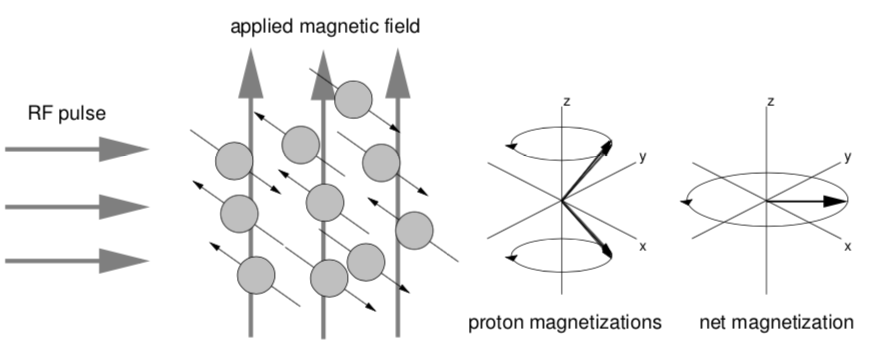
\includegraphics[width=0.8\textwidth]{rfpulse}
\end{figure}

\ix{Relaxation Mechanisms}There are different mechanisms which restore equilibrium:
\begin{enumerate}
  \item $T_2$ relaxation is `spin-spin' relaxation caused by \ix{$T_2$ relaxation}de-phasing of the precessing vectors. Spinning protons generate tiny fields which \emph{randomly} effect the fields of the neighbours, reducing the net magnetisation. The time constant depends on the material. 
  \marfig{t2relax}{}

  \item\emph{Non-random }$T_2^*$ relaxation however dominates where de-phasing occurs due to magnet imperfections, variations in the magnetic susceptibility of the patient and small scale field inaccuracies. The time constant of this decay is \emph{at least} an order of magnitude smaller than that of $T_2$.

  \item$T_1$ relaxation also occurs concurrently with the $T_2$ process where protons revert from their excited state to the parallel state until equilibrium is restored with energy dissipated into the latice. The time constant is material dependent (though increasing with field strength) but always longer than $T_2$ . 
  \marfig{t1relax}{}
\end{enumerate}
As the spins relax a \emph{signal with frequency proportional to the strength of the magnetic field} is emitted.

Thus an MRI scanner seeks to measure the proton density in the material (which affects signal strength) as well as the $T_1$ amd $T_2$ time constants with:\ix{MRI Components}\marfig{mrisetup}{}
\begin{itemize}
  \item A magnet to product a strong, uniform and steady field.
  \item A RF transmitter.
  \item A gradient system which produces \emph{time varying magnetic fields of controlled spatial non-uniformity}.
  \item Some detection and imaging system. 
\end{itemize}
Referring to the diagram alongside, the output signal is due to the component of the net spin vector in the $x-y$ plane. 

\ix{Spin-Echo Sequence}We are unable to use free induction decay because this decays too fast due to the $T_2^*$ relaxation. In order to resolve this problem, the \textbf{spin-echo} sequence is used during which an additional RF pulse corresponding to phase shift $\pi$ is used after the original pulse. This pulse flips all the spins over meaning that the spins now come back into phase meaning the `echo' recovers to where it would have been if only $T_2$ decay acts (after which the signals dies).

\ix{Spin-Echo - Diagrams}
\begin{figure}[H]
  \centering
  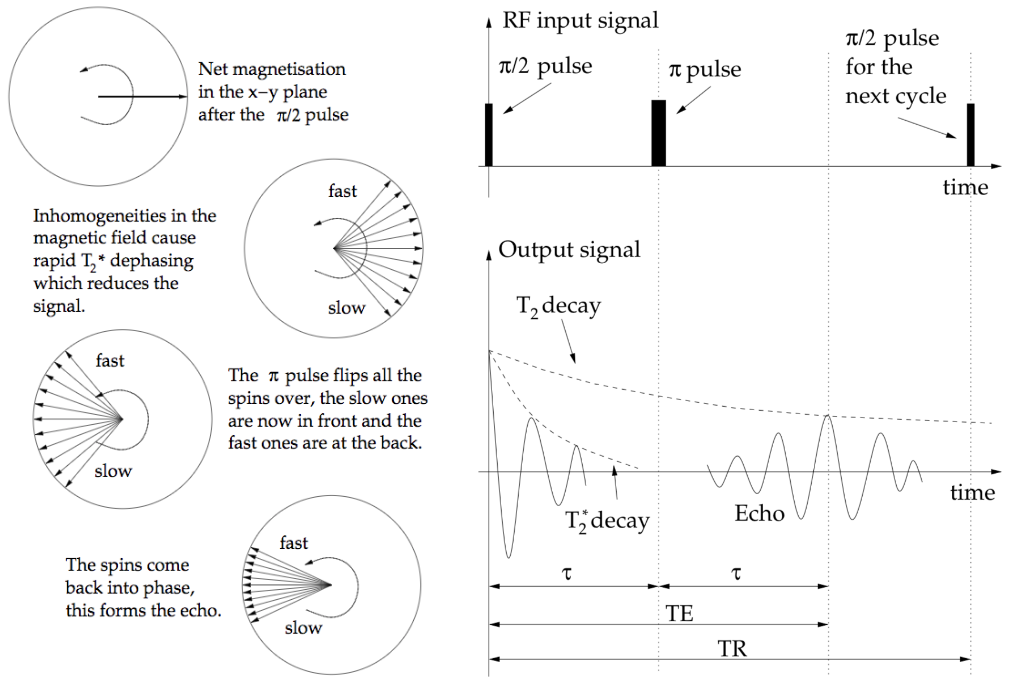
\includegraphics[width=\textwidth]{spinecho}
\end{figure}

\ix{3D Spatial Encoding}For 3D spatial encoding, three constraints are required:\marfig{3denc}{}
\begin{enumerate}
  \item Slice selection: the gradient field settings set a plane with the Lamor frequency of the RF pulse frequency. 
  \item Gradient settings are applied for a short time to set spin phases to different values at different points. 
  \item Further gradient settings are used during readout to generate \emph{frequency encoding} during reception. 
\end{enumerate}

\marfig{imagetypes}{Image Weighting}
Different weightings are possible for images which then affect the output image; please see table right. 

\section{Extracting Information from 3D Data}
\subsection{Surface Representations}
Surface representations allow volume data such as CT datasets to be displayed more intuitively. We will mostly consider representing surfaces as either polygonal meshes or parametric bicubic patches. 

Polygons are 2D surface primitives defined by an ordered list of vertices. By convention, the polygon normal (defined by the right hand rule) points outwards from the front face. Neighbouring polygons must have consistent ordered. Polygonal meshes can be represented in different ways but there tends to be a tradeoff between memory usage and ease of manipulation (e.g.\ consider lists of shapes vs vertices vs edges).\ix{Establishing mesh consistency} In order to establish the consistency of a mesh, we require that:
\begin{itemize}
  \item Polygons are closed and planar.
  \item Vertices are appropriately ordered. 
  \item Edge vertex is referenced by two edges. 
  \item Edges are not reused within a polygon.
  \item Polygons do not self intersect.
\end{itemize}
Whilst the edge scheme is the easiest to check for consistency\ix{Which scheme is used in practice?} it can create further inconsistencies (e.g.\ non-edge connected polygons) and thus vertex lists are used as a common trade off. 

\ix{Finding Polygon Normals}Polygon normals are essential. A robust approach used to find polygon normals is to find a plane close to each of the vertices:
\begin{align*}
  Ax + By + Cz + D = 0
\end{align*}
where \emph{the areas of the polygon projected onto the axis planes determine the plane coefficients} e.g.
\begin{align*}
  A = \frac{1}{2}\sum_i (z_i + z_{i \bigoplus 1}) (y_i + y_{i \bigoplus 1}
\end{align*}
$D$ can be determined by inserting a vertex into the plane equation. 

Many polygons are required to represent a curved surface; bicubic patches offer a good alternative. Considering curves, we use a\ix{Why parametric and cubic?} parametric, cubic representation since this allows us to get multiple values of $y$ for a given $x$ (unlike $y(x)$) and it is easy to join curves. A third order polynomial is a good compromise in providing flexibility without introducing extra computation and thus four 3D constraints are required to specify a curve.\ix{Formulation} Limiting the range of $t$ to $[0,1]$, we form

\begin{align*}
  \underbrace{
  \begin{bmatrix}
    x(t) & y(t) & z(t)
  \end{bmatrix}}_{\vect{Q}(t)} = 
  \underbrace{
  \begin{bmatrix}
    t^3&t^2& t& 1
  \end{bmatrix}}_{\vect{T}}
  \underbrace{
  \begin{bmatrix}
    a_x &a_y& a_z \\
    b_x& b_y &b_z \\
    c_x &c_y &c_z \\
    d_x &d_y &d_z \\
  \end{bmatrix}}_{\vect{C}} \\
\end{align*}

Curves are joined by connecting segments at $t=1$ to another where $t=0$. The curves have $G^0$ \emph{geometric} continuity if they meet and $G^1$ continuity if the tangent vector \emph{directions} are equal (usually sufficient for CAD). They have $C^1$ \emph{parametric} continuity if the tangent magnitudes are equal; if up to $d^n\vect{Q}(t)/dt^n$ is equal, the curves have $C^n$ parametric continuity. $C^2$ continuity is normally required for camera paths in animation. \marfig{contin}{Continuity of Curves}

The convex hull of a set of points in the set of points which may be written as a linear sum of the points with the weights all in $[0,1]$ and summing to one. \marfig{conhull}{Convex Hull}

\ix{Matrix Decompositions}We normally write \(\vect{Q=TMG}\) i.e \(\vect{C=MG}\). \(\vect{M}\) is a $4 \times 4$ basis matrix and \(\vect{G}\) is a $4 \times 3$ geometry matrix. We can also write \(\vect{Q=BG}\) to emphasise that the curve is a weighted sum of elements from the geometry matrix. There are different forms of cubic curves:\ix{Curve Types}
\begin{enumerate}
  \item Hermite curves are determined by position constraints and tangent vectors of the endpoints. 
  \begin{figure}[H]
    \centering
    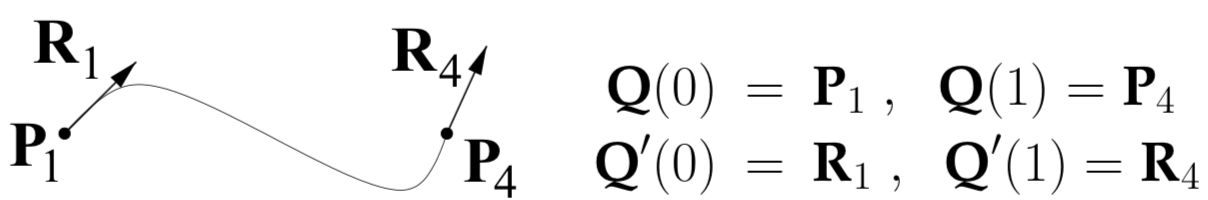
\includegraphics[width=0.6\textwidth]{hermite}
  \end{figure}
  It is straightforward to join these curves with $G^1$ continuity.

  \item Bézier curves are similar to the Hermite form except that the tangents are defined by points $\vect{P_2, P_3}$\marfig{bezier}{}

  The geometry matrix can be found via substitution into the Hermite form where the tangents include a factor of $3$ i.e. $\vect{R_1} = 3\vect{(P_2 - P_1)}$ to give a constant parametric velocity for four equally spaced control points. These curves \textbf{satisy the convex hull property} which can be proven by examining the blending 
  functions.  

  \item The B-spline has a geometry matrix made up of four points where $C^2$ continuity can be achieved by sharing three control points between adjacent curve segments. The line only approximates the control points but the convex hull property is satisfied. B-splines can be transformed in an affined manner by transforming the control points. 

  \begin{figure}[H]
    \centering
    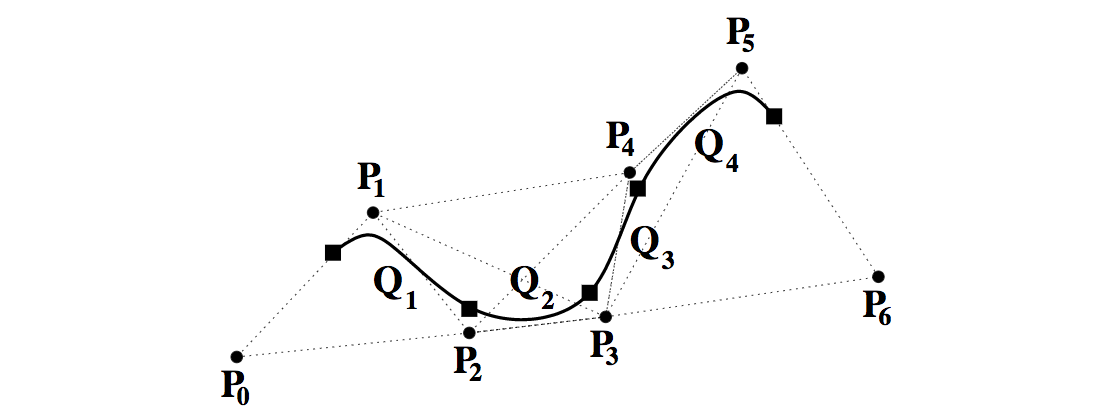
\includegraphics[width=0.6\textwidth]{bspline}
  \end{figure}

  \item The Catmull-Rom splines are similar to b-splines but they pass through the two control points and the remaining points determine the tangent vectors. These splines have $C^1$ continuity but not the convex hull property. 
  
\end{enumerate}


In general, it is\ix{Forming the \(\vect{C}\) matrix} possible to form the \(\vect{C}\) matrix by forming four constraints in a matrix and applying matrix inversion.  \ix{Converting between forms}It is also straightforward to convert between different forms by setting \(\vect{TM_bC_b=TM_sG_s}\) and inverting matrices to give the new geometry matrices.

Curves\ix{Subdivision} can be subdivided where the same curve is represented using several segments in order to provide more flexibility. If repeatedly subdividing, the control points form a better and better approximation for the curve. \marfig{repsub}{Repeated Subdivision}It is easiest to divide Bézier curves, followed by Hermite curves. 

Since it is easy to convert between different forms of curves, it is only necessary to consider which form to \emph{define} curves.\ix{Defining curves: Key Questions} We ask whether we want an approximator or interpolant, whether to define the curve using points, whether we desire the convex hull property and what continuity is required.

Curves are converted into patches by including an additional parameter
\begin{align*}
  \vect{Q}(s, t) = \vect{SMG}(t)
\end{align*}
i.e. \(\vect{G}\) is a function of $t$; fixing $t$ gives a cubic curve in $s$ and the set of surfaces sweep a patch. \ix{General form of a bicubic patch}Considering each axis separately, 
\begin{align*}
  x(s,t) &= \vect{SMG}_x(t) \text{ where } \vect{G}_x^T = \vect{TMQ}_x^T \\
  \therefore x(s,t) &= \vect{SMQ}_x\vect{M}\vect{T}^T
\end{align*}
where \(\vect{Q}_x^T\) is a \(4\times 4\) geometry matrix. \ix{Understanding the Geometry Matrices}The meaning of the \(\vect{Q}_x^T\) matrix can be understood e.g. for a Hermite patch by noting that \(\vect{G}_x(t)\) takes form of the Hermite geometry matrix in which each point itself follows a cubic paths in $t$. 

Each curve type discussed before can be extended to a patch type.\begin{enumerate}
	\item Recalling the form of Hermite curves, the meaning of \(\vect{Q}_x\) can be understood; they encode the positions of the patches corners, tangents at the corners (in both the $s$ and $t$ directions) as well as the \emph{twists} at the corners. \ix{Joining Hermite Patches}Hermite patches can be joined with $C^1$ continuity if the positions, tangents and twists of the shared edges are identical. 
	
	\item Similarly, \ix{Bézier Patches} Bézier patches can be expressed by note that the sixteen elements of each geometry matrix define a net of sixteen control points; the four control net corners lie on the patch with each boundary curve defined by a Bézier curve with boundary control points. When joining these patches, $C^0$ continuity is possible by making the four shared control points equal and $G^1$ continuity occurs when the two sets of four control points on either side of the common edge are collinear with the edge control points. Note that the convex hull property holds.   
	
	\item \ix{B-spline Patches}The geometry matrices of B-spline patches define sixteen control points. In general, none of these points are interpolated though the convex hull property is preserved. If the control points are shared in the usual way (and \emph{not} duplicated), $C^2$ continuity is guaranteed. 
\end{enumerate}

\ix{Evaluating the Surface Normal}The surface normal at any point is easy to calculate
\begin{align*}
\vect{n} = \frac{\partial \vect{Q} }{\partial s} \times \frac{\partial \vect{Q} }{\partial t}
\end{align*}
where each vector terms can be obtained using straightforward derivatives. 

\marfig{subpat}{Subdividing Patches}Patches may be subdivided by extending the procedure for subdividing curves; this can provide a polygonal approximation to a cubic surface (i.e. using the control points) which is useful for graphics hardware which is optimised for polygons. However, if there are regions of high curvature resulting in the use of non-uniform subdivision, tears may arise between patches which are divided to different degrees. There is not a significant cost in subdividing the entire patch in a uniform cost so this is the usual approach. 

\newpage
\subsection{Surfaces and Interpolation of Sampled Data}
Medical imaging techniques produce \emph{voxel arrays} which are generally not useful for visualisation; in general, surfaces produced by thresholding the data are far more useful for visualisation and if the data values have an absolute meaning, is an appropriate and meaningful technique e.g. CT data. However, note that data from other sources may only depict \emph{relative} properties. Even in appropriate cases, the voxel data often represents spatial averages of meaningul properties which can cause issues such as partial voluming e.g. around tissue-bone boundaries, the voxel data will be representative of neither tissue nor bone. \marfig{partvol}{Partial Voluming}

Morphological operations may be applied to scalar-valued data:
\begin{itemize}
	\item \textbf{Erosion} replaces each pixel with the minimum of its neighbours, thinning an object.
	\item \textbf{Dilation} replaced each pixel with the maximum of its neighbours, thus fattening an object.
\end{itemize}
Neighbours are defined using a \emph{mask} centered on the current pixel. e.g.
\begin{figure}[H]
	\centering
	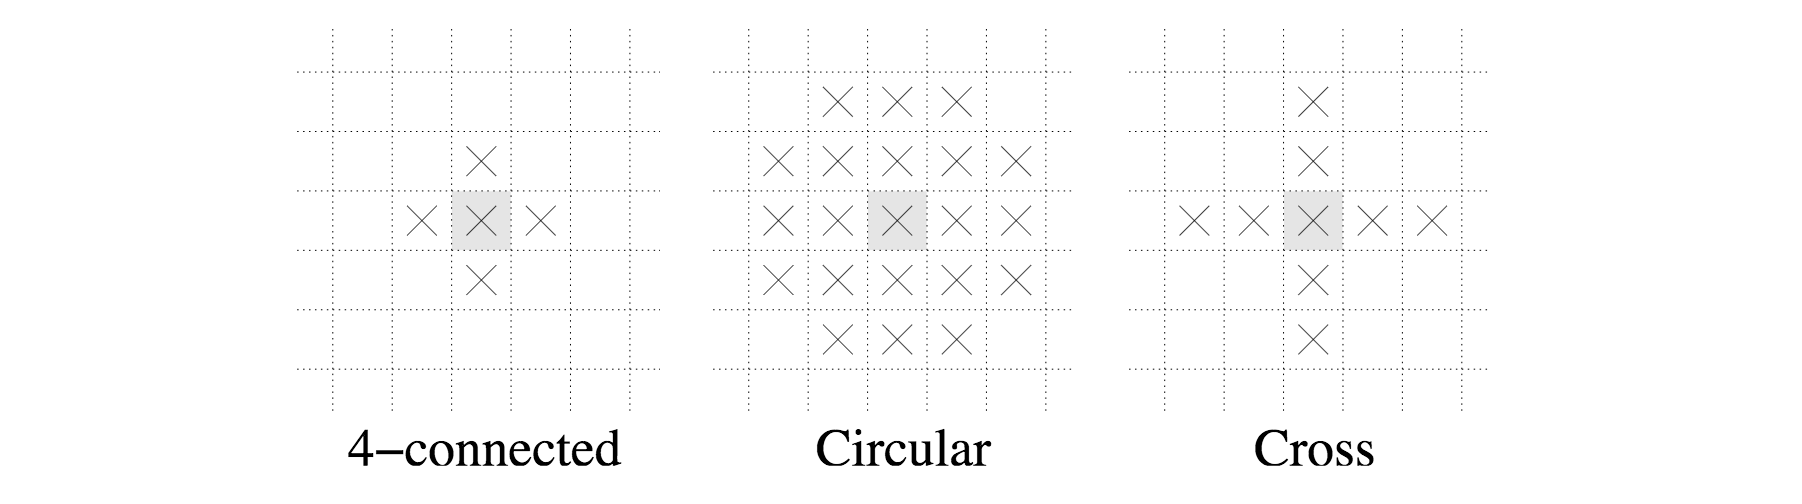
\includegraphics[width=0.9\textwidth]{masks}
\end{figure}
The 4-connected mask ensures 4-connected objects, the cross preserves horizontal and vertical lines while the circular mark smooths the object boundary. \ix{Morphological Operations}Approximately the same number of erosions and dilations are used to give an approximately equal size. Opening operations are $N$ erosions are followed by $N$ dilations (which tends to remove small objects and object links) whilst closing is the opposite. 

\ix{2D Contouring}An simple method for extracting a 2D contour is \emph{contour following} where a contour is followed and relevant edges labeled until the initial edge is returned too (after which a new seed is chosen) leading to the three cases found right \marfig{confol}{}. A polyline may then be drawn which passes through the edges midpoints (which improves the perimeter estimate since otherwise diagonals are overestimated by $\sqrt{2}$). Contours may reach the edge of the image, in which case a choice from the following is made:
\begin{itemize}
	\item Arbitrarily classify the region outside the image. All contours will be closed and linked.
	\item Halt at the border, return to the seed and then follow the contour in the other direction. 
	\item Only track \emph{closed} contours that are fully connected within the image. 
\end{itemize}
Note however there is an ambiguity \marfig{conamb}{Contour Ambiguity}and whichever implementation is chosen, pixels of one class are 4-connected whilst the other class is 8-connected. 

An alternative to contour following is the \ix{Marching Squares}marching squares algorithm which can be implemented in parallel where (if scalar data is available), the location of the contour can be interpolated, providing a far better estimate of the contour area. 
\begin{figure}[H]
	\centering
	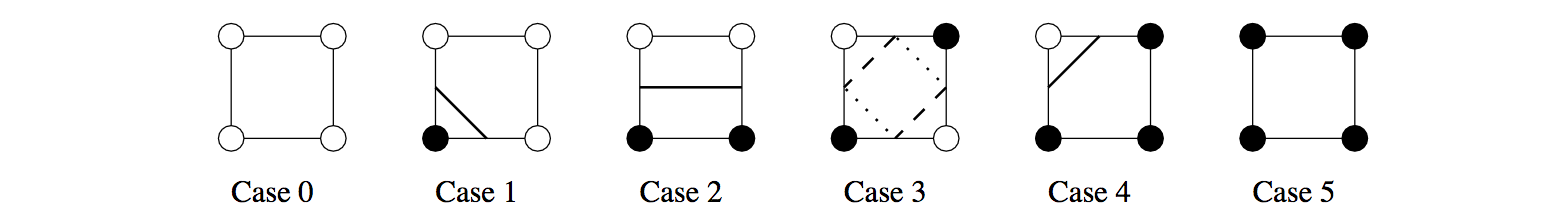
\includegraphics[width=0.9\textwidth]{marsqa}
\end{figure} 
Note the ambiguity in case (3). \ix{Calculating the Contour Area}The area of the contour may be calculated as follows:
\begin{align*}
 A = \frac{1}{2}\sum_n \vect{v}_n \times  \vect{v}_{n\bigoplus1}
\end{align*}
\marfig{conare}{}i.e. by summing contributions from triangles connecting each edge to the origin. Note that the area is \emph{signed} and the summation represents the area swept out an odd number of times.

 \ix{Marching Cubes}Marching cubes is a 3D isosurface generating algorithm analagous to 2D marching squares with 256 states (reduced to 15) where a lookup table is used to generate the appropriate polygons (triangle strips). Care must be taken when choosing the ambiguous states to ensure continuous surfaces which do not self-intersect (i.e. manifold). Often marching cubes generating too detailed meshes which are subsequently decimated. The enclosed volume of the surface can be calculated by summing \emph{signed} volume contributions over triangles. \marfig{tetvol}{}
 \begin{align*}
 V = \frac{1}{6}\sum_t (\vect{a} \times \vect{b})\cdot \vect{c}
 \end{align*} 
This requires consistent vertex ordering and well-behaved surface (as defined above). The above formula can be proved by noting that $A_i = \frac{1}{2}|\vect{a \times b}|$ and the height is given by $\vect{n\cdot c = \frac{\vect{a \times b}}{|\vect{a \times b}|}}\cdot\vect{c}$ where each vector is between some arbitrary point and the triangle vertex. 

If space is tesselated with tetrahedra rather than cubes, \ix{Marching Tetrahedra}only two cases are required which require polygonisation and the second only requires a quadrilateral. There are also no ambiguous cases though there are more triangles than with marching cubes and we must be able to sample on a tetrahedral grid. Tetrahedra can be aligned with a rectangular grid (e.g. using a body-centred cubic lattice) but this may require interpolation. 

\ix{Mesh Decimation}Often surfaces can be represented well using a smaller number of triangles than an algorithm such as Marching Cubes produces e.g. consider flat surfaces. Mesh Decimation is used to simplify redundant meshes, reducing the number of triangles. The algorithm works as follows:
\begin{enumerate}
	\item Preserved vertices lying on feature, boundary or non-manifold edges. 
	\item Calculate a measure of the (local) error introduced by removing each vertex.
	\item Remove vertices which have small errors and then retriangulate. 
\end{enumerate}
Retriangulation may be performed using edge collapse or other techniques (e.g. pure removal, vertex merging) and results in a mesh with a consistent surface accuracy. The aspect ratios of each triangle may be improved after mesh decimation which can make the surfaces look better.

A major issue is that we do not know how the underlying function behaves between sampled points. We attempt to either interpolate or approximate to form a continuous function. Since approximators are less constrained, it is easier to find smooth approximating functions. There are several techniques for interpolation/approximation:
\begin{itemize}
	\item Nearest\ix{Nearest Neighbour Interpolation} neighbour interpolation sets the function value to value of the nearest voxel. Whilst simple, it results in visible block artifacts (unless the voxels have size similar to the display pixels). 
	\item Linear interpolation\ix{Linear Interpolation} constructs the value function at each point using linear weights from either of the neighbouring points. This method is \emph{separable} i.e. the interpolation can be performed in each dimension in turn (and thus is efficient). 
	\item B-splines\ix{B-spline Approximation} can be adapted to approximate a scalar function of three parameters\marfig{bsplineapp}{} defined by 64 control points (the data values in a $4\times 4\times 4$ voxel neighbourhood) evaluated inside the 8 central voxels. The approximation may serve to smooth noise and the convex hull property ensures the function is constrained within the voxel values that define the spline. 
\end{itemize}
In fact, B-splines can be used to render isosurfaces directly from the volume data without an intermediate polygon representation; this is known as volume rendering. 

In reality, volume data is unlikely to be isotropic (e.g. with CT scans, the slice spacing is typically 2-3mm whilst resolution within a slice is sub-millimetre). Interpolation can \ix{Shape-Based Interpolation: Motivation} be used to generate intermediate slices but linear interpolation can lead to step artefacts in isosurfaces so \emph{shape-based interpolation} is used to interpolate between sets of binary data sets which gives smoother isosurfaces. The method for this is as follows:\ix{Method}
\begin{enumerate}
	\item Calculate the distance transform for each contour on the known slices.
	\item Interpolate the \emph{distance transform} between slices e.g. linearly. 
	\item Form the intermediate isosurface from the zero-contour of the intermediate distance field. 
\end{enumerate}

The\ix{Distance Transform} is used to compute a distance field for each contour. Positive distances are inside the contour and negative distances outside. A naive solution would be to calculate the distance from each image pixel to each contour point but this is $\mathcal{O}(n^2)$. The distance transform is an  $\mathcal{O}(n)$ algorithm which uses a local estimate of the data as follows:\ix{The Distance Transform Algorithm}
\begin{enumerate}
	\item Initialise the image so pixels next to the edge (in a 4-connected sense) have values set to $\pm 5$ and all other pixels set to large values e.g. $\pm 100$.
	\item Use either the \emph{City-Block} or \emph{Chamfer Masks} to examine each pixel. In the forwards pass, process left to the right and top to bottom and replace the centre pixel with the \emph{smallest absolute magnitude} from the mask combined with the data.
	\begin{figure}[H]
		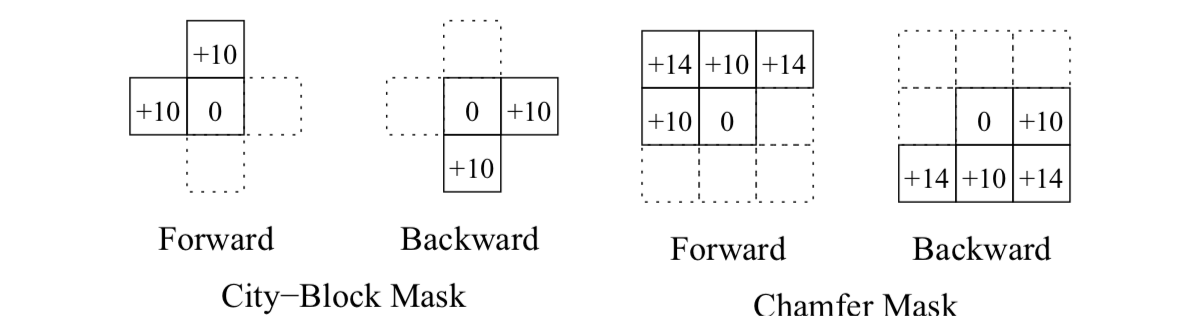
\includegraphics[width=0.7\textwidth]{dsmask}
		\centering
	\end{figure}
    \item Calculate values for the edges (where the masks are unable to reach). 
\end{enumerate}
The chamfer mask is more complex but gives a better distance estimate (effectively allows diagonal shortest routes). They represent the distance to the contour is constrained to walk along the paths defined by each mask. Distance\ix{Uses of Distance Transforms} transforms are used for geometry assessment (e.g. generating an object skeleton), expanding an object (3D transforms to enlarge radiotherapy targets) and to measure the alignment between two objects (e.g. by adding the distance transforms).  

Unstructured data is difficult to interpolate and is produced often by freehand scanners or geophysical imaging. One approach is to directly form a mesh using the \emph{Delaunay Triangulation}\ix{Delaunay Triangulation} which has the following properties:
\begin{itemize}
	\item In 2D, the minimum interior angle of a triangle in the Delaunay triangulation is greater than (or equal to) the same angle for any other triangulation. 
	\item It is the \emph{dual} of the Dirichlet tesselation (which is a tiling where each tile covers the space closest to a point). 
	\item The circumsphere of any $n$-dimensional simplex contain no other points except the defined simplex points. (An $n$-dimension simplex is a convex region defined by $n+1$ independent points). e.g. in 2D, the circumcircles of each triangle enclose the triangle vertices. 
\end{itemize}
\begin{figure}[H]
	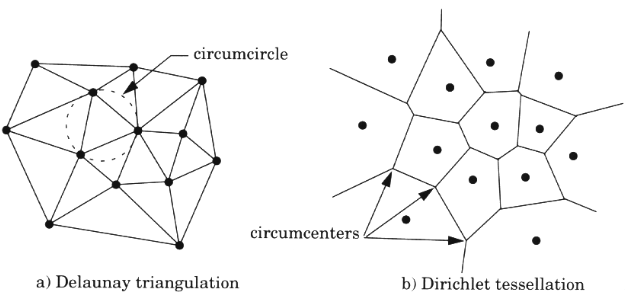
\includegraphics[width=0.7\textwidth]{deltri}
	\centering
\end{figure}
\ix{Algorithm}In order to add a new vertex:
\begin{enumerate}
	\item Add a new vertex. 
	\item Delete any triangle which has a circumcircle that strictly contains the new vertex, creating a hole in the mesh. 
	\item Add new triangles to the mesh, each defined by the new vertex and an adjacent pair of vertices on the hole boundary. 
\end{enumerate}
The algorithm is initialise with a single triangle then iterated ($\mathcal{O}(n^2)$) but a more subtle algorithm can give $\mathcal{O}(n\log n)$. This results in a mesh which spans the convex hull of the initial point set but note that this does not produce a unique mesh. This structure can then be used for interpolation. This method is poor at handling highly irregular and sparse data. 

\ix{RBF Interpolation}An alternative is \textbf{RBF Interpolation}. This takes the form
\begin{align*}
s(\vect{p}) = p_m(\vect{p}) + \sum_{i=1}^n \lambda_i \phi(||\vect{p}-\vect{p}_i||_2) \hspace{1cm} \vect{p} \in \mathbb{R}^d, \lambda_i \in \mathbb{R}
\end{align*}
\begin{itemize}
	\item $\vect{p_i}$ is an interpolation node (and hence a location where the function is known).
	\item $\phi(\cdot)$ is some fixed function (the RBF). The choice of function is important and will determine the form of the eventual function. \marfig{rbf}{}Commonly used choices are linear, $r^2 \log r$ (thin-plate spline), Gaussian $\exp[-ar^2]$ or multiquadratic $\sqrt{r^2+c^2}$.
	\begin{figure}[H]
		\centering
		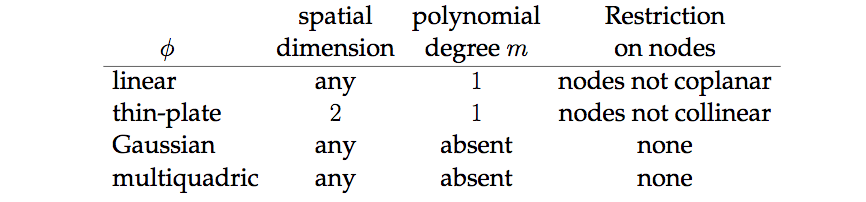
\includegraphics[width=0.7\textwidth]{rbftab}
	\end{figure}
	\item Each $\lambda_i$ is a weight for each interpolant node (to be determined). 
	\item $p_m$ is some polynomial of degree $m$ (which is typically small) with coefficients which must be determined. The polynomial degree is chosen to ensure an invertible linear set of equations. This is often referred to as the trend function as far from the interpolation nodes, $s$ is dominated by this polynomial. 
\end{itemize}
In order to find the coefficients\ix{Finding the Unknowns}, we require two conditions:
\begin{enumerate}
	\item The RBF should interpolate the function values. 
	\begin{align*}
	s(\vect{p_i}) = f(\vect{p_i}) \hspace{1cm} i = 1, \ldots, n
	\end{align*} 
	
	\item The coefficients should be unique. 
	\begin{align*}
	\sum_i \lambda_i q(\vect{p_i}) = 0 \hspace{1cm} \forall q \in \pi_m^d
	\end{align*}
	where $\pi_m^d$ is the space of all polynomials in $d$ variables which degree $\leq m$. e.g. if $d=2, m=1$ this requires that 
	\begin{align*}
	\sum_i \lambda_i x_1 = \sum_i \lambda_i x_2 = \sum_i \lambda_i = 0 
	\end{align*}
\end{enumerate}
These constraints can be written in matrix form and subject to the constraints before, the matrix is guaranteed to be invertible. e.g. with $d=2, m=1$ the $N+3 \times N+3$ interpolation matrix takes the form\ix{Interpolation Matrix}
\begin{align}
\begin{bmatrix}
\phi(|| \vect{p_1} - \vect{p_1}  ||_2) & \cdots & \phi(|| \vect{p_1} - \vect{p_n}  ||_2) & 1 & x_1 & x_2 \\
\vdots & & \vdots & \vdots & \vdots & \vdots \\ 
\phi(|| \vect{p_n} - \vect{p_1}  ||_2) & \cdots & \phi(|| \vect{p_n} - \vect{p_n}  ||_2) & 1 & x_n & x_n \\
1 & \cdots & 1 & 0 & 0 & 0 \\
x_1 & \cdots & x_n & 0 & 0 & 0\\
y_1 & \cdots & y_n & 0 & 0 & 0\\
\end{bmatrix} 
\begin{bmatrix}
\lambda_1 \\ \vdots \\ \lambda_n \\ c_0 \\ c_1 \\c_2
\end{bmatrix} 
= 
\begin{bmatrix}
f_1 \\ \vdots \\ f_n \\ 0 \\ 0 \\0
\end{bmatrix} 
\end{align}
\ix{RBF Performance}Note that
\begin{itemize}
	\item The RBF interpolant tends to degrade gracefully with few artefacts. 
	\item RBFs are suited to problems with a smooth and continuous underlying function; the thin-plate spline provides $C^1$ continuity and higher order splines better this. 
	\item \ix{Space and Time Complexity}For large $n$, the storage and inversion of the interpolation is difficult and numerical techniques are used even though the condition number can be hard. Brute force requires $\mathcal{O}(n^3)$ operations and $\mathcal{O}(n^2)$ in space but new techniques can avoid starting again if only a few extra nodes are added; this requires $\mathcal{O}(n \log n)$ operations and $\mathcal{O}(n)$ in space.
    \item Evaluation of the RBF is $\mathcal{O}(n)$ but faster incremental methods have evolved. 
    \item \ix{Dealing with Noisy Data}With noisy data, the interpolation constraints can be relaxed to allow the RBF to approximate the function. 
    \item For time varying signals (with fixed nodes), each new set of readings requires a simple matrix multiplication (and thus the costly matrix inversion is avoided). 
    \item Vector fields can be interpolated; the system is solved one and each additional component requires a matrix multiplication to determine the appropriate parameters. 	
\end{itemize}

\ix{Plugging Gaps using RBFs}The technique is also useful in other areas; e.g. if parts of skull are missing, a patchy surface from a B-spline approximation can be represented as a scalar field, $z=f(x,y)$. RBF interpolation can be used with a support region around the hole edge. Sampling across a fine mesh can allow the surface to be estimated.

\subsection{Direct Surface Capture}
As an alternative to capture volume data and creating isosurfaces, it is possible to directly capture surface data\ix{Real World Examples} which finds use in computer animation, medicine (e.g. plastic theory) as well as industry (rapid prototyping). Whilst passive methods such as computer vision are finding some use, the most popular method are laser range finders. The principles of laser scanning are:\ix{Principles of Scanning}
\begin{itemize}
	\item A surface is scanned using a laser beam and is observed with a camera. 
	\item The \emph{relative positions} of the laser source and camera are known. 
	\item Either triangulation or time-of-flight is used to determine the range. 
	\item Scanning either occurs mechanically or free hand. 
	\item Surfaces are represented as point clouds.
\end{itemize}

\marfig{laser}{}Refering to diagram right, $L, \theta, \phi\ \&\ f$ are fixed by the scanning geometry and the camera. For each point $P$ we seek the depth, $Z$, which is calculating using the location of $P$ on the image plane. $Z$ can be expressed as a function of $x$ using simple geometry. In order to scan more of the surface, either the laser (and cameras) or the subject must move which limits the maximum size. \ix{Limiting the Size}Alternatively, freehand systems exist which are portable, cheap and flexible. 

\ix{Problems with Laser Beams}However, each observation only provides information about a single point on the surface meaning a scan will take time. Instead, the surface is often scanned using a stripe of laser light which can be produced by passing the beam through a cylindrical collimating lens. \marfig{stripe}{}Each point on the image of the line $x'$ can be triangulated to locate a point on the surface.

Scanning isn't perfect; common problems include\ix{Scanning Problems}
\begin{itemize}
	\item Self-occlusion occurs e.g. noses on faces. this can be resolved using additional cameras. 
	\item Deep cavities are difficult to scan and additional cameras won't help. The object can be dissected into more complex parts but if this is not possible a gaps remain (which can be patched over e.g. using RBF interpolation). 
	\item Edge curl produces artifacts at sharp corners (or at colour boundaries) due to the finite width of the laser beam which causes discontinuities in the computer mesh. \marfig{curl1}{}
	\begin{figure}[H]
		\centering
		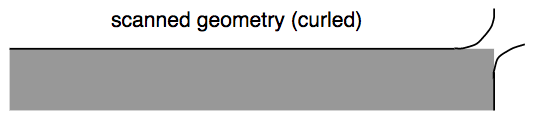
\includegraphics[width=0.5\textwidth]{curl2}
	\end{figure}
	\item Multiple reflections cause translucent, transparent surfaces .
	\item Speckle occurs due to interference of laser light due to surface microstructure (but this is normally fine). 
	\item Object motion can cause problems if the scanning time is long. 
	\item Ambient lighting.
	\item The resolution which the angle of reflection, $\alpha$, is measured at is fixed by the resolution of the cameras CCD. As a result, the \textbf{depth resolution decreases as the scanned object is further from the scanner}.\marfig{lasdepres}{}
\end{itemize}

Space encoding allows for faster acquistion of range data where $2^N$ discrete lines are imaged with only $N$ video frames by projecting a series of binary patterns in sequence onto the subject which recursively subdivide the FoV into two. The cubicscope uses the same principle but rotating mirrors are used to sweep a pulsed laser across the surface. Care must be taken with the exposure time of the camera. Also note that an additional camera can be used to provide texture maps.  

\begin{figure}[H]
	\centering
	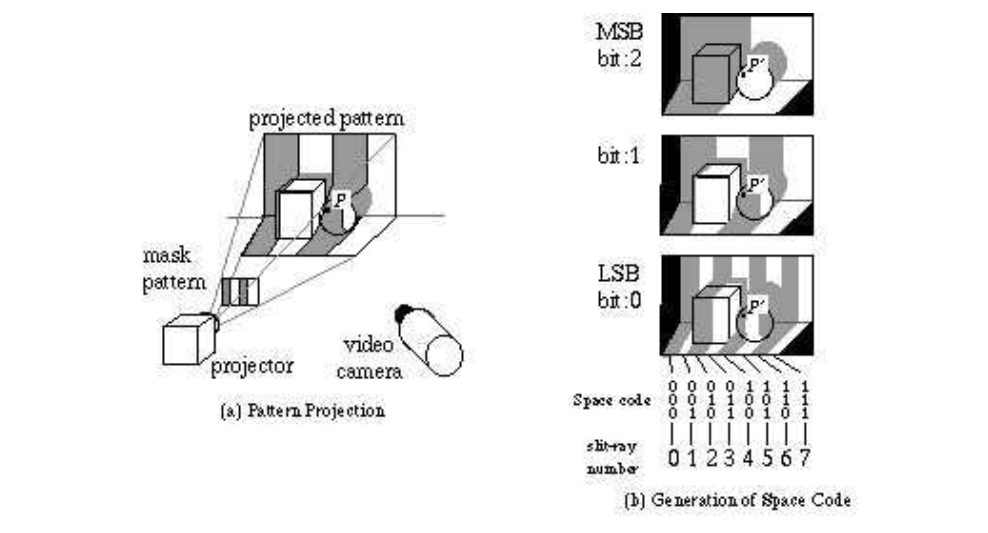
\includegraphics[width=0.8\textwidth]{spaceencoding}
\end{figure}
Each of the video camera's pixels has an associated illumination code which identifies the source of the incident light. A look-up-table is then used to speed up the computation of range data. Over long distances, time-of-flight ranging is useful but this technique is made more difficult due to dispersion. 

\ix{Forming a Mesh}In general, adjacent points are not necessarily adjacent on a surface passing through them and forming a mesh from a set of points is difficult. The line of sight of the laser tells us which side of each point the object lies. The point cloud from mechanical scanners is arranged regularly and thus the vertices can be joined to generate triangular strips but for free-hand systems this performs poorly. For this unstructured data, RBF interpolation can be used to fit a 3D function to the point set with a zero-isosurface which corresponds to the surface. The same techniques can then be used as for volume data. When a large surface is scanned,\ix{Scanning Large Surfaces} the meshes need to be merged but there are bound to be \emph{registration errors} between the patches (e.g. slight misalignment). If RBF interpolation is used, this can be resolved by merging vertices rather than meshes and then using a single RBF interpolation (where the RBF is used to \emph{approximate}) the data. 

\section{3D Computer Graphics}
\subsection{Surface Rendering}
Medical imaging normally produces volumetric data which can either be displayed directly using volume rendering or converted into surface polygons and patches which are then rendered using surface rendering. \ix{Surface Rendering: Motivation} We seek to go from sets of bicubic patches or polygons and produce a realistic, shaded rendering of it. 

\ix{Surface Rendering Pipeline}The surface rendering pipeline takes in polygon vertices (along with other properties such as those of the surface, camera and lighting). Note that other effects are involved such as texturing and fog. \texttt{OpenGL} is an open source graphics library used extensively. The pipeline can be split into a number of sub-processes:
\begin{enumerate}
	\item Objects are modelled in their own, local coordinate systems. 
	\item Objects are then embedded into a world coordinate system. Lighting sources, viewpoint and camera properties are defined.
	\item Objects are transformed into view coordinates (back face culling may occur here).
	\item The polygons are transformed into 3D screen space and clipped to the view volume. 
	\item The polygons are mapped onto discrete coordinates in 2D device coordinates (rasterisation). Hidden surface removal occurs and a reflection model colours each pixel. 
\end{enumerate}
\ix{Dealing with Bicubic Patches}Note that bicubic patches are usually rendering by splitting the patch into polygons. 
\begin{figure}[H]
	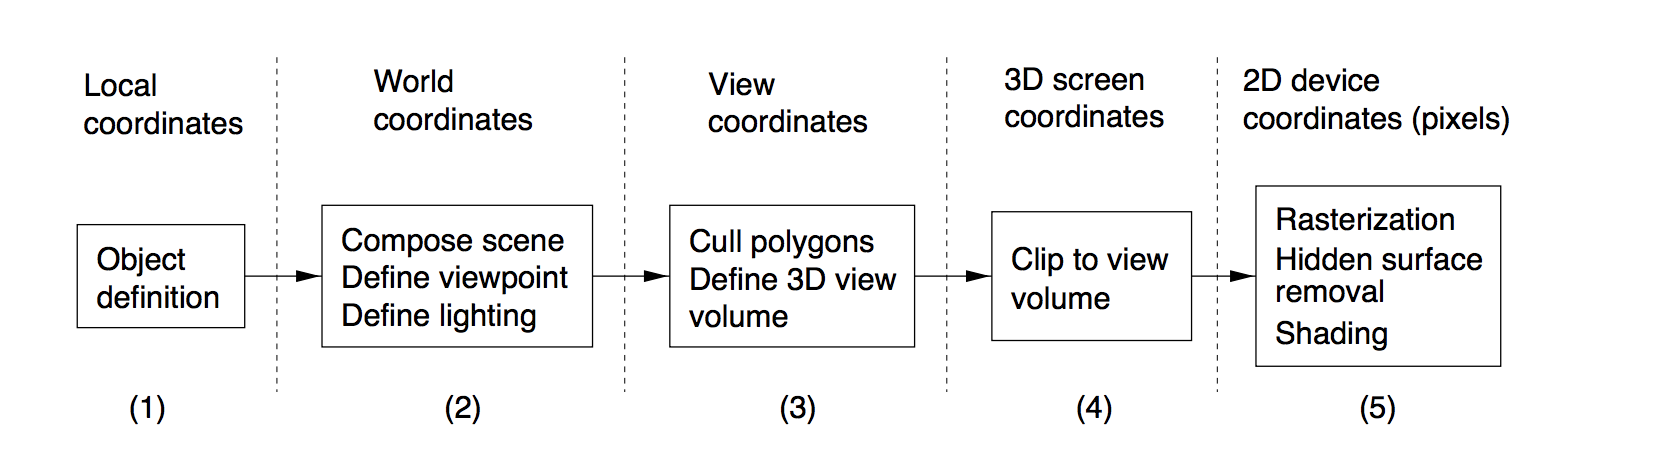
\includegraphics[width=0.9\textwidth]{surfacepipeline}
	\centering
\end{figure}


\subsubsection*{Stages 1 \& 2: Composing the Scene}
The rigid body transformation between local coordinates and world coordinates\ix{Local to World Coordinates} is described by a rotation matrix and vector. Thus in homogenous coordinates, this transform is equivalent to simply multiplying by the \emph{modelling matrix}.

\ix{Defining the Viewpoint}The position of the camera is specified by the world coordinates of the centre of projection. The orientation is then defined by the view plane normal (direction) and a view up vector (whose orthographic projection onto the view plane gives the $y_v$ axis). \marfig{defview}{}There are 10 degrees of freedom in specifying the camera properties:
\begin{enumerate}
	\item 3 DoF in specifying the camera centre of projection.
	\item 3 DoF in specifying the VPN and the VUV.
	\item 4 DoF in the view volume (see next section). 
\end{enumerate}Thus world to view coordinates is another rigid body transformation and the transformation between local and view coordinates is known as the \emph{modelview matrix}. In practice, a more complex system known as PHIGS is used which has more degrees of freedom since the view volume is not assumed to be symmetric. 

\subsubsection*{Stages 3 \& 4: World Coordinates to 3D Screen Coordinates}
\marfig{perproj}{Perspective Projection}Perspective projection is used to transform view coordinates into 3D screen coordinates. This produces realistic images since it results in \emph{foreshortening} where distant objects appear smaller. This is achieved by finding the intersections between the view plane and rays connecting the object and the centre of project. \textbf{Note that the }$z_v$ \textbf{ axis points backwards along the viewing direction} to ensure a right handed coordinate system.  Similar triangles show that
\begin{align*}
x_p = \frac{-dx_v}{z_v} \hspace{1cm} y_p = \frac{-dy_v}{z_v}
\end{align*}

A view volume is defined\ix{View Volume: Motivation} by a near and far plane as well as a rectangular window in the view plane. This is desirable since\marfig{viewclip}{View Volume Clipping}
\begin{itemize}
	\item Distant objects would appear very small in the image (and thus may cause aliasing issues).
	\item Nearby objects would appear too large; they may obscure other objects.
	\item Moving the near plane allows simple reslicing. 
	\item Objects behind the camera should be ignored. 
\end{itemize}
Note that clipping the view volume is difficult; each vertex must be tested against each clipping plane. Thus the coordinates are normalised give the full set of 3D screen coordinates.
\begin{align*}
x_s = \frac{x_p}{x_{\text{max}}} \hspace{1cm} y_s = \frac{y_p}{y_{\text{max}}} \hspace{1cm} z_s = \frac{f(1+ n/z_v)}{f-n}
\end{align*}
Note that the transformation from $z_v \rightarrow z_s$ is \textbf{non-linear} but ensures that lines in view coordinates are lines in screen coordinates. \textbf{Lines on the same projector has the same} $(x_s, y_s)$.

\ix{Homogenous Coordinates}We use homogenous coordinates (e.g. to express the above transformations) as they minimise floating point division and allow all transformations to be represented as matrix multiplications which are hardware accelerated e.g. a transformation and rotation ($\vect{T}$ and $\vect{R}$ respectively) can be expressed as
\begin{align*}
\begin{bmatrix}
wx \\ wy \\ wz \\ w
\end{bmatrix}
=
\begin{bmatrix}
 &  &  &  \\ 
 & \vect{R} &  & \vect{T} \\ 
 &  &  &  \\ 
0 & 0 & 0 & 1 \\ 
\end{bmatrix}
\begin{bmatrix}
x \\ y \\ z \\ 1
\end{bmatrix}
\end{align*}
Note that orthographic projection (sometimes useful e.g. scientific visualisation) can also be represented using homogenous coordinates; the underlying equation are
\begin{align*}
x_s = \frac{x_v}{x_{max}} \hspace{1cm} y_s = \frac{y_v}{y_{max}}
\hspace{1cm} z_s = \frac{z_v + n}{n-f}
\end{align*} 
Since the homogenous coordinates are normalised, floating point operations are minimised by clipping vertices directly in these coordinates, for example, $ |wx| \leq w$; this is far easier than clipping with the viewing planes. \emph{Polygon clipping}\ix{Polygon Clipping} is more subtle than this since a polygons vertices may need revising. The \emph{Sutherland-Hodgman} algorithm clips the polygon against each infinite plans of the view volume in turn by traversing a polygon's set of vertices and outputting a set of vertices. 
\begin{figure}[H]
	\centering
	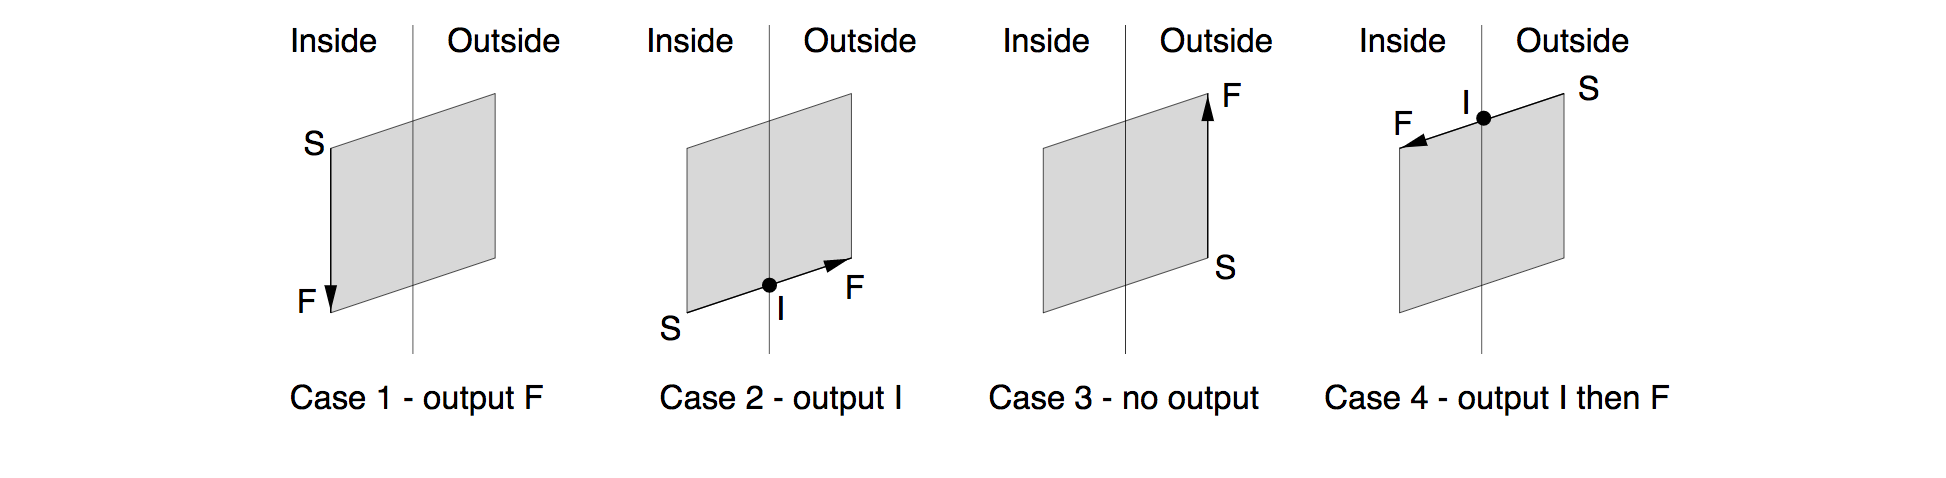
\includegraphics[width=\textwidth]{polyclip}
	The algorithm can be implemented recursively (call itself from an outputted vertex). 
\end{figure}

\ix{Back-Face Culling}Back face culling removes polygons which the camera cannot see (note: this can be done before the transformation to 3D screen coordinates). If the polygon ordering has been defined such that when viewed from the front, the vertices are anticlockwise, the normal (determined using the corkscrew rule) can be found. \marfig{cull}{} If there are no reflections (and under other conditions), polygons with surface normals pointing away from the camera cannot be visible. Such polygons are identifying by taking a dot product between the normal and any vector from the centre of projection to the polygon. Note that there are other hidden surfaces (e.g. hidden `ledges' which are removed later in the pipeline). Culling is only effective with \emph{solid} polyhedra and sensible clipping planes. 

\subsection{Illumination, Reflection \& Shading}
Here, simple illumination and reflection models (allowing intensities of light to be recorded from a point) are developed in order to give feasible shading algorithms (converting the above information to intensities and colours for the \emph{screen pixels}). We focus on \emph{local models}\ix{Assumptions Made} which consider only direct illumination and \textbf{not} light reflected from other surfaces. Point light sources are also assumed. This gives significant efficiency gains at the cost of realism. 

\ix{Characterising Surface Reflections}The \emph{bidirectional reflectivity function} is used to characterise surface reflections. \marfig{bdrf}{}
\begin{align*}
R_{bd}(\lambda, \phi_i, \theta_i, \phi_v, \theta_v) = \frac{I_v(\phi_v, \theta_v)}{E_i(\phi_i, \theta_i)}
\end{align*}
Note the dependence on the wavelength of light, $\lambda$. Emperically, two behaviours are observed:\ix{Reflection Types}
\begin{enumerate}
	\item A specular response is where light is mostly reflected in the `mirror direction'. The surface would appear shiny in a local reflection model and act as a mirror in a global model. 
	\item Diffuse reflections have their response spread over a larger range of angles generally with a bias in a particular reflection (not necessarily the mirror direction). 
\end{enumerate}
Note that there is a dependence on $\theta_i$; grazing angles of incidence often give specular behaviour. 
%diagram for the different reflection types

The \ix{Phong Reflection Model}Phong reflection models give a good first order approximation to photo-realism which has become \emph{de facto} for most applications. 

\begin{align*}
I_\lambda = \underbrace{c_\lambda I_a k_a}_{\text{Ambient}} + \sum_i f_{\text{att}} I_{p,i} (\underbrace{c_\lambda k_d \vect{L}_i \cdot \vect{N}}_{\text{Diffuse}} + \underbrace{k_s (\vect{R}_i \cdot \vect{V})^n )}_{\text{Specular}} \\
\text{where  }\lambda \in \lbrace r, g, b\rbrace, \hspace{1cm} f_{\text{att}} = \min \Big (\frac{1}{a_1 + a_2 d + a_3 d^2}, 1 \Big )
\end{align*}
Note that:\ix{Explain the Phong Model}
\begin{itemize}
	\item Colours are modelling by calculating the equation for each colour. The colour of the object is itself modelling using the values of $c_\lambda$.
	\item $\vect{N}$ is the \emph{visible} surface normal.
	\item $k_d$ is a diffuse reflection coefficient (other constants similar). 
	\item The $\cos \theta$ in the diffuse terms accounts for more specular reflection at larger angles. 
	\item $\vect{R_i}$ is the mirror direction (a function of the illumination direction, $\vect{L}$ and the normal).
	\item The larger $n$ is, the more shiny the object (since the specular reflection will decay quicker with $\alpha$).
	\item Note there is no $c_\lambda$ term for specular reflection; in the real world, the colour of specular highlights is dominated by the colour of the light source and thus the light source colour is used.  
	\item Ambient light of intensity $I_a$ is added to the model to prevent surfaces turned away from the source being invisible. $k_a$ is the a surface dependent ambient reflection coefficient. 
	\item An attenuation factor is included so surfaces with the same orientation but differences in distance to the light source are not assigned the same intensity. The form is due to the \emph{inverse square law} but other terms are included to compensate for the point light source assumption.
	\item The summation over $i$ is a summation over multiple light sources.  
\end{itemize}

\subsubsection*{Stage 5: Rasterisation, Shading and Hidden Surface Removal}
\ix{Rasterisation}Rasterisation is the conversion of a polygons screen coordinates to discrete pixel coordinates. Clearly the array should have the same aspect ratio as the window in the view plane; this conversion is straightforward e.g. 
\begin{align*}
x = 0.5(x_s + 1) \cdot (x_{\text{right}} - x_{\text{left}}) + x_{\text{left}}. 
\end{align*}
However, converting edges into pixels is not straightforward. A polygon filling approach suffices for 3D graphics where for every edge of the polygon, one $x$ value is found for every $y$ value. A simple algorithm to do this is from the edge coordinates $(x_1, y_1), (x_2 y_2)$ is.  

\begin{algorithm}[H]
	\caption{\label{alg:ascent}Simple Rasterisation}
	\begin{algorithmic}[1]
		\State $x \gets x_1$
		\State $m \gets (x_2 - x_1)/(y_2 - y_1) $
		\For{$y=y_1 \textbf{ to } y_2 $}
			\State $\text{output(round(} x \text{), } y \text{)}$
			\State $x \gets x + m$ 
		\EndFor
	\end{algorithmic}    
\end{algorithm}

This algorithm can be reformulated to only use integer arithmetic and avoid floating point operations. (See examples paper or try this for yourself). \ix{Storage}Rasterised polygons are stores as \textbf{linked lists} of spans.\marfig{raster}{}The pixels between alternate pairs require shading but if the polygon is convex, there is only even one span meaning that the $x$ values need not be sorted. 

\ix{Correcting the Sizing Problem}Unfortunately, rasterised polygons tend to be bigger than the actual polygons. This is remedied by applying the following rules:
\begin{enumerate}
	\item Discard horizontal edges. 
	\item Edges which run from $y_1$ to $y_2$ should generate x-values from $y_1$ to $y_2 - 1$. 
	\item Scan lines should only be shaded from $x_1$ to $x_2 - 1$.
\end{enumerate}

\ix{Shading Models}It is incredibly expensive to apply the Phong model to every pixel; faster alternatives are used included:
\begin{itemize}
	\item Flat Shading: the Phong model is used to calculate a colour of one pixel on each polygon. The entire polygon is then shaded with this colour. (Note that calculating at the vertices and interpolation only gives a marginal improvement). This makes the polygon structure very obvious. 
	
	\item Gouraud Shading: the surface normal at each vertex of the mesh is estimated by averaging the normals of neighbouring polygons. \ix{When is Vertex Smoothing a bad idea?}The vertex smoothing degrades rendering when the mesh does actually represent the shape of the object (can be remedied by subdivision). \marfig{vertint}{} The colour of each vertex are then calculated using the Phong model and interpolation is used to get colours for interior pixels. Note that the interpolation can be done using fast, incremental calculations (since it must be done for each pixel, this is especially easy for the final scan line - linear interpolation occurs across a single line and thus $I_{p,n} = I_{p, n-1} + \Delta I_p)$. 
	
	The linear interpolation used is an approximation for the Phong reflection model and is especially poor with the specular component (if the specular reflection is at the centre of an object, it will be missed). 
	
	\item Phong Shading: vertex normals are calculated and these \textbf{normals are interpolated}\marfig{phongshade}{} which tends to restore the original curvature of a surface.  
	
	Even though incremental calculations can be used, this method is very expensive and each normal has three components. Then a separate intensity if calculated for each normal. Modern graphics hardware (with \emph{fragment/pixel shaders}) can implement this shading at interactive rates. 
\end{itemize}

The final process within stage 5 is hidden surface removal; the most common approach is known as the \emph{z-buffer algorithm}\ix{Z-Buffer Algorithm}. 
\begin{enumerate}
	\item Calculate the $z_s$ value for each pixel by linearly interpolating stored values for polygon vertices. 
	\item The pixel intensities are stored in the frame buffer; initialise the z-buffer to have the same dimensions and all values set to the maximum depth.
	\item For each polygon, calculate the intensities and update the z-buffer and frame buffer if $z<z_{\text{buffer}}$ i.e. if the new polygon is in front of whatever was in the old buffer. 
\end{enumerate}
Normally there is one rendering algorithm which does rasterisation, shading as well as hidden-surface removal. \ix{Overall Rendering Algorithm}

\begin{algorithm}[H]
	\caption{\label{alg:render}Rendering Algorithm with Gouraud Shading}
	\begin{algorithmic}[1]
		\State Set all z-buffer values to the maximum depth.
		\State 
		\For {each polygon}
		\State Calculate vertex normals and intensities. 
		\State Calculate $x, z, I$ for each scan line $y$ and store them in \texttt{EdgeList(y)}
		\EndFor
		\State
		\For {$y=y_{\text{min}} \texttt{ to } y_{\text{max}}-1$}
		\For {$\text{segment in }\texttt{EdgeList}(y)$}
			\State {get $x_l, x_r, z_l, z_r, I_l, I_r$ from \text{segment}}
			\For {$x=x_l \texttt{ to } x_r - 1$}
			\State {\text{calculate} z, I \text{by interpolation}}
			\If {z<\text{z-buffer(x, y)}}
				\State {$\text{z-buffer}(x, y) = z$}
				\State {$\text{frame-buffer}(x, y) = I$}
			\EndIf
			\EndFor
		\EndFor
		\EndFor
	\end{algorithmic}    
\end{algorithm}

\ix{Parametric Surfaces}Note that parametric surfaces (e.g. bicubic patches) are rendering by converting patches into polygonal meshes by subdividing the curves until each sub-patch satisfies some flatness condition. 

\subsection{Advanced Topics}
\subsubsection*{Shadows}
The \ix{Shadow Z-Buffer Algorithm}shadow z-buffer algorithm is a algorithm used to add shadows to the standard rendering pipeline. \begin{enumerate}
	\item Render the scene using the light source as the view-point, only filling in a shadow z-buffer. At the end of this process, this contains the distance from the light-source to the \emph{nearest polygon} along each ray. 
	
	\item Render the scene using the intended view point. If a point is visible, convert it's 3D screen coordinates to the screen coordinates \emph{as seen from the light source}. Compare the converted $z_s'$ to the stored value, $z_b$. If $z_b < z_s'$ then there is a surface between the point and the light source and the point is rendered with a reduced illumination. 
\end{enumerate}

\ix{Dealing with Aliasing}A problem is that a single view plane pixel does not map onto a single pixel in the shadow z-buffer. Thus pixels may be in partial shadow but if we only use one $z_b$ value this will give aliasing effects. Thus calculate transformed coordinates for each of the pixels four corners (which defines some quadrilateral in the shadow z-buffer) allowing the fraction of the pixel in shadow to be deduced which can be used to get a suitable attenuated illumination intensity. 

\ix{Multiple Light Sources}Note that it is easy to generalise this technique to multiple light sources by having several shadow z-buffers for each light source and adding a shadow fraction term, $S_i$, to the Phong model. 

\subsubsection*{Texture Mapping}
Texture mapping modifies surface colours by wrapping a 2D image onto a surface in order to enhance realism.\ix{Texture Mapping} Each texture is defined as $\vect{T}(s, t)$ and to apply the mapping, each polygon vertex is associated with a point on the texture map. The colours of the points inside the polygon are found by interpolation the texture coordinates between the vertices using \textbf{perspective interpolation} which takes depth into account.\marfig{texmap}{} This is widely supported on commodity graphics hardware. 

\ix{3D Texture Mapping}3D texture mapping is also supported in hardware but requires a lot of texture memory. A similar procedure is followed to above but if $(s, t, r) = (x_l, y_l,z_l)$ 3D texture mapping can be thought of as carving an object using a chunk of solid material with the given 3D texture. 

Textures for natural objects e.g. wood, granite or marble can be algorithmically generated. 

\subsubsection*{Global Illumination Models}
\ix{Recursive Ray Tracing}Recursive ray tracing is a technique used which allows for indirect illumination. It accounts for hidden surface removal, transparency effects and shadow computation at once. A ray, $\vect{V}$, is fired from the centre of projection through \emph{every pixel on the screen} and further rays are spawned when objects are hit:
\begin{enumerate}
	\item One ray, $\vect{L}_i$ heads for the $i$th light source (and if it passes through objects, the illumination intensity is attenuated).
	\item A reflection ray, $\vect{M}_i$ is spawned.
	\item A refraction ray, $\vect{T}_i$ is spawned with the direction determined by Snell's law. 
\end{enumerate}
\marfig{raytrace}{}The intensity of the pixel is calculated
\begin{align*}
I_\lambda = c_\lambda I_a k_a + \sum_i S_i f_{\text{att}} I_{p,i} (c_\lambda k_d \vect{L}_i \cdot \vect{N} + k_s (\vect{R}_i \cdot \vect{V})^n ) + k_s I_{r\lambda} + k_t I_{t\lambda}
\end{align*}
\ix{Why recursive?}where the values of $I_{r\lambda}$ and $I_{r\lambda}$ are found by recursive evaluation at the surfaces which are next intersected using the original point of contact as the view point. Thus a \emph{ray tree} is followed and constructed \emph{top down} until a ray fails to intersect an object or some maximum depth is is reached. Evaluation then occurs \emph{bottom up}. \marfig{raytree}{}

\ix{Evaluating Recursive Ray Tracing}The algorithm works but is very expensive and have some aliasing problems. Note that the algorithm can be mapping to parallel hardware. Ray tracing models give only specular reflection and refraction and thus images produced are unmistakeably shiny. 

\subsubsection*{Volume Rendering}
An alternative to the surface rendering pipeline, volume rendering is an alternative to viewing volumetric data. \ix{Intuition}It can be thought of as taking an X-ray of the the voxel array. Each voxel is assigned $\lbrace c_r, c_g, c_b, \alpha \rbrace$ i.e. a colour and an opacity. This technique is often used in conjunction with front and back clipping plans to limit the portions of voxel array which are used for a single image. Note that this is quite expensive and only recently has it become feasible on the available hardware. 

\ix{Rendering Algorithm}A ray is fired from each pixel in the image plane to the view volume and the intensity of the ray is updated at each voxel intersection. \marfig{volrend}{}The final values of $I_{\lambda, \text{out}}$ sets the pixel colour. Note that transparent voxels ($\alpha = 0$) don't affect the intensity and opaque voxels stop contributions from further down. There are also issues with aliasing artifacts. 

Setting $\alpha$ and $c_\lambda$ is not easy. If the volumetric data was CT data, each voxel could be classified by looking at the CT number and then a different colour could be assigned to each type of materials (e.g. air vs bone vs fat). The rendering quality can be improved by including some local reflectance by looking for local surfaces and calculating their colours using the Phong model. Note that if the volumetric data is $v$, the surface normals are aligned with $\nabla v$. 

\ix{Evaluation}Volume rendering is highly interactive with the user setting the viewing angle, clipping planes, material classification thresholds, colours and opacities for each material, surface detection and reflection properties. An expert operator is required but volume rendering can be very impressive. 

\subsubsection*{Graphics Processing Units}
Graphics software is written either using \texttt{Direct3D} or \texttt{OpenGL} and all computers contain graphics hardware which implement functions in each library directly. Important hardware components are:\ix{GPU Hardware Flow}
\begin{enumerate}
	\item \textbf{Vertex Shaders} which take input vertices and transform them into output vertices under the control of a user-defined program. 

	\item Other dedicated hardware performs clipping and mapping to 2D device coordinates. 
	
	\item Clipped vertices are assembled into primitives (usually triangles) before a rasterizer interpolates the vertex data to give pixel data. 
	
	\item Fragment/pixel shaders use the interpolated data and run another user-defined program to produce pixel outputs e.g. Phong shading. Texture mapping occurs at this stage. 
\end{enumerate}
Shaders are written in either \texttt{HLSL (Direct3D)} or \texttt{GLSL (OpenGL)}; custom shaders are not essential but they can give advanced rendering effects. 

\ix{GPUS in General}In general, GPUs have larger number of operations per second than CPUs with many operations occurring in parallel (which works since vertices are independent until the framebuffer). 

\subsubsection*{Volume Rendering by Texture Mapping}
Volume rendering can be performed at interactive\ix{Performing Volume Rendering at Interactive Rates} rates by exploiting the dedicated GPU hardware to perform this rendering as 3D texture mapping. The voxel array is defined as a 3D texture field and if there is enough memory, the entire voxel array can reside on the GPU which gives very fast rendering. \textbf{Blending} the intensities from back to front is essential to simulate transparency.

If there isn't sufficient memory for the texture, similar results can be obtained by reslicing the data and mapping the reslice images onto the polygons as 2D textures. 



\end{document}